\graphicspath{{anexos/AnexoF-Recopilacion-Soluciones-Por-Fases/recursos/}}

\section{Recopilación de las Soluciones de cada Caso} \label{Anexo:recopilacion-soluciones-por-fases}

En este anexo recopilamos para cada caso las figuras que representan visualmente:
\begin{enumerate}
	\item La planificación inicial, previa a los cambios debido a la incidencia
	\item La solución inicial, resultado de la \faseuno{}.
	\item La solución final, resultado de la \fasedos{} empleando VNS. 
\end{enumerate}


\newpage
\subsection{Caso 1}

\begin{figure}[!h]
	\centering
	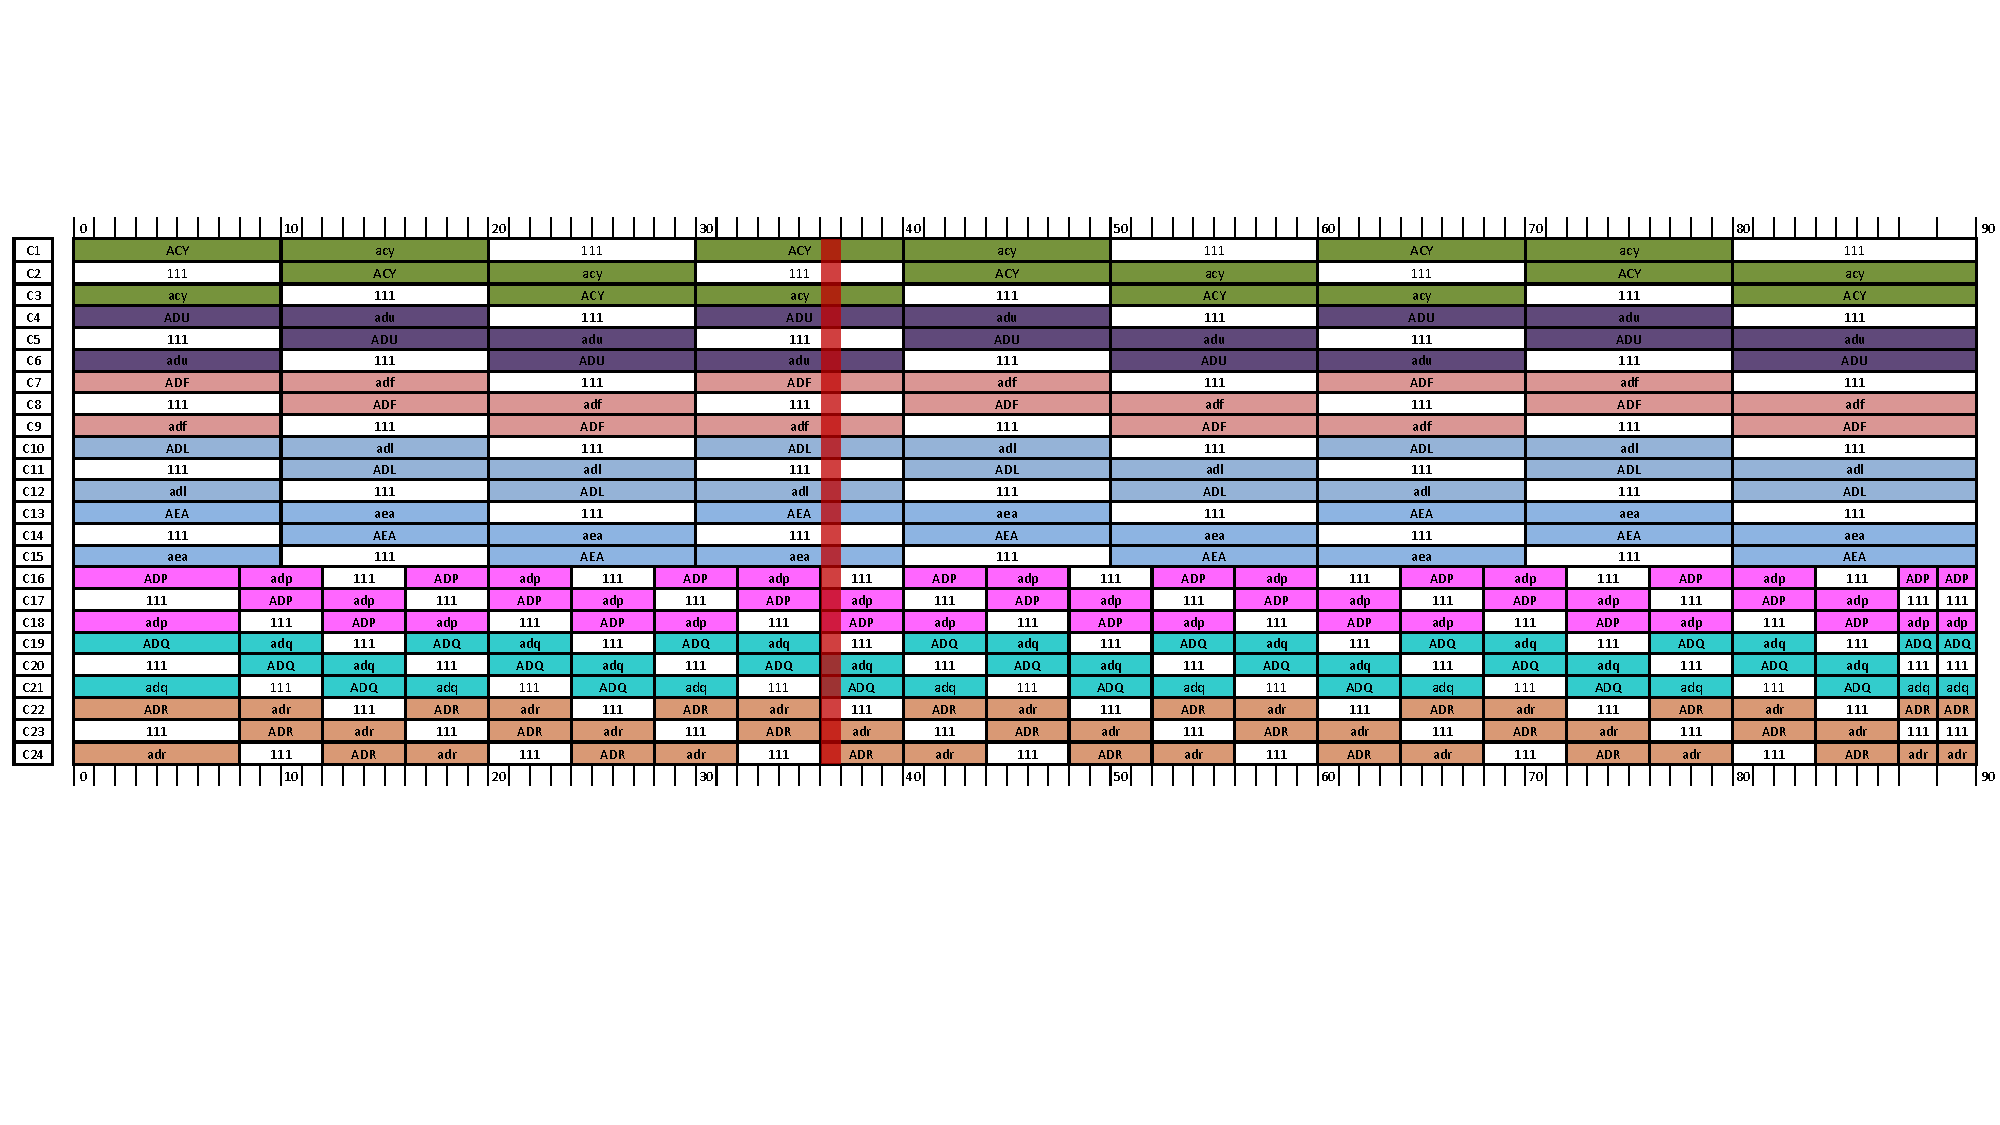
\includegraphics[width=\linewidth]{caso1/caso1-fase0}
	\caption{Planificación inicial del Caso 1}
	\label{fig:caso1-fase0}
\end{figure}

\begin{figure}[!h]
	\centering
	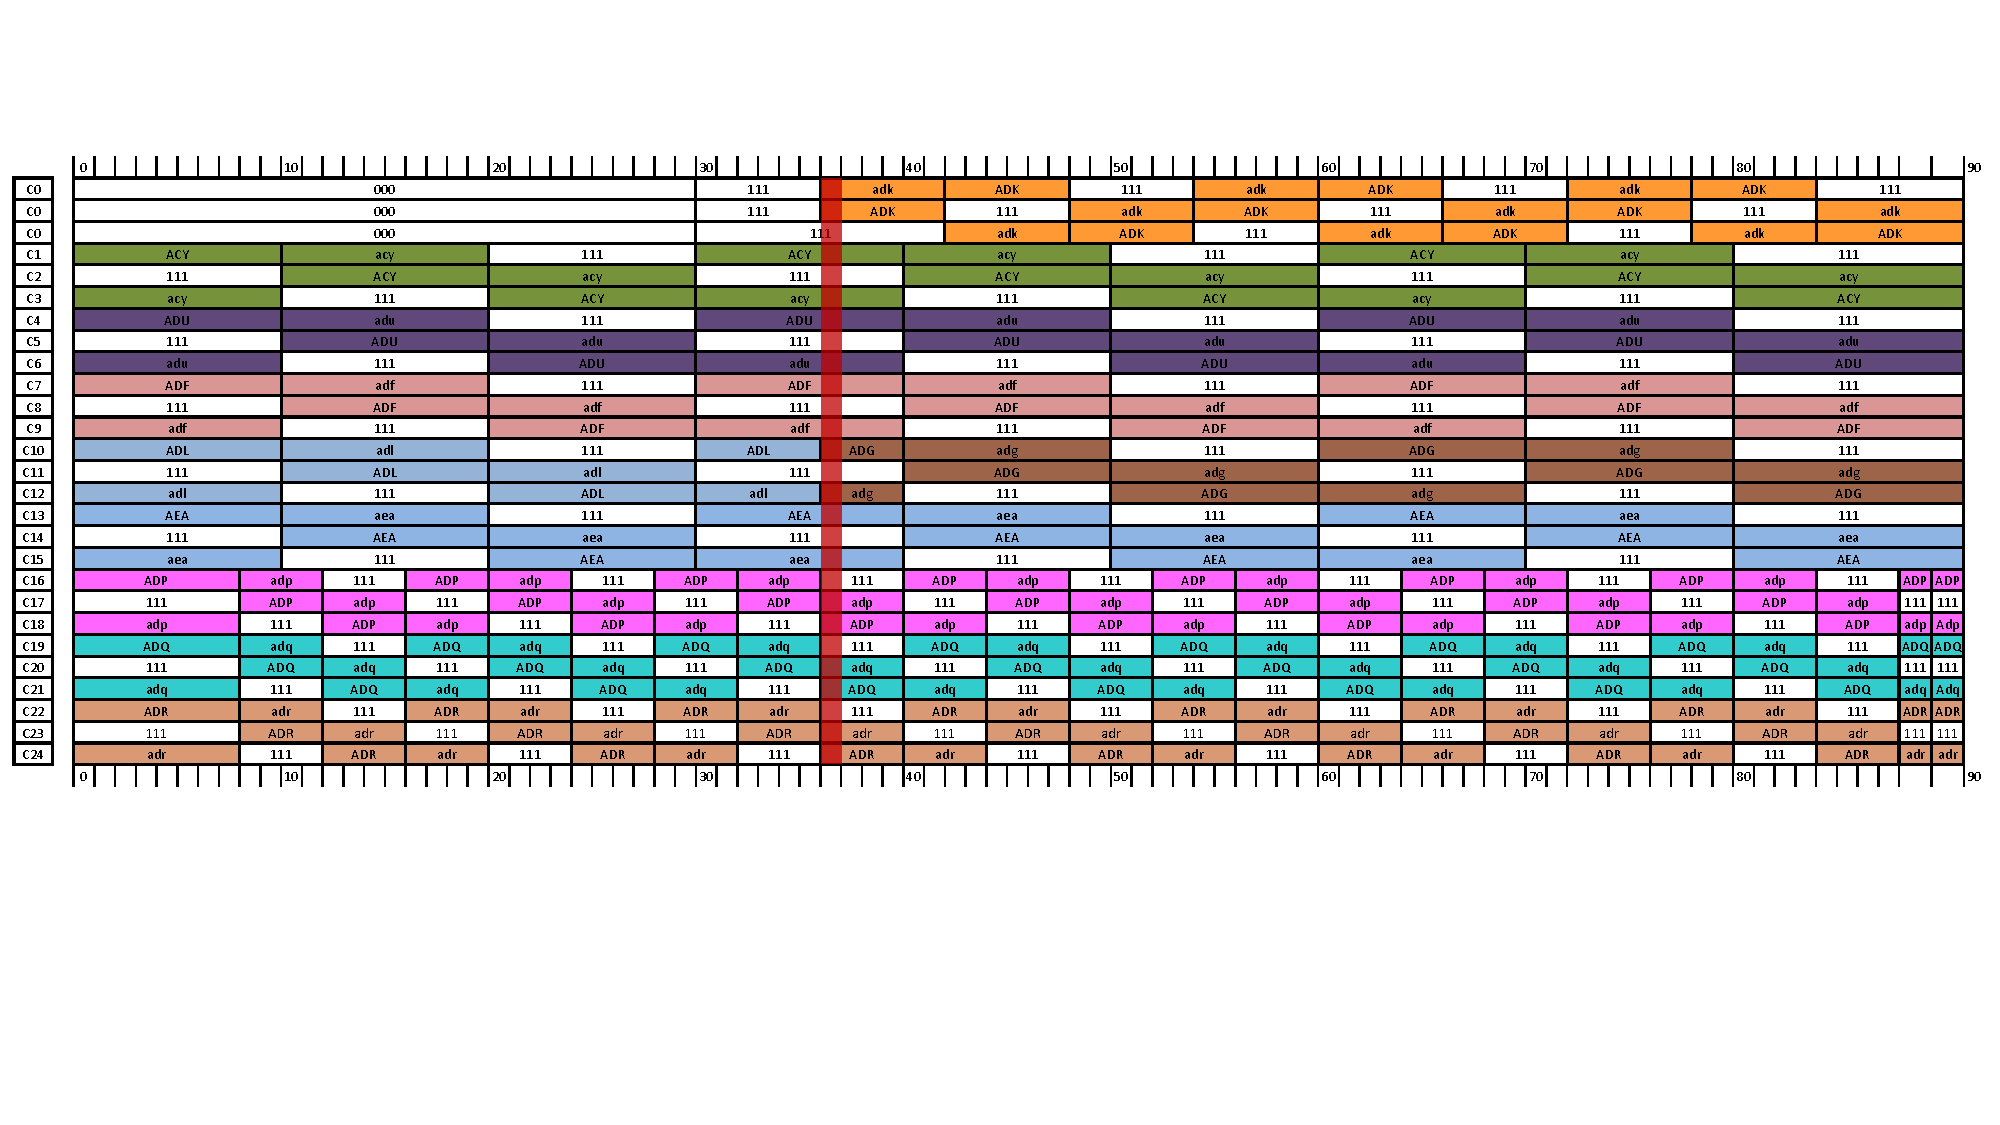
\includegraphics[width=\linewidth]{caso1/caso1-fase1}
	\caption{Solución inicial (\faseuno{}) para el Caso 1}
	\label{fig:caso1-fase1}
\end{figure}

\begin{figure}[!h]
	\centering
	\includegraphics[width=\linewidth]{caso1/caso1-fase2-vns}
	\caption{Solución final (\fasedos{}) para el Caso 1}
	\label{fig:caso1-fase2}
\end{figure}

\FloatBarrier
\newpage
\subsection{Caso 3}

La planificación inicial es la misma que la del Caso 1, cambiando el slot del momento del cambio.

\begin{figure}[!h]
	\centering
	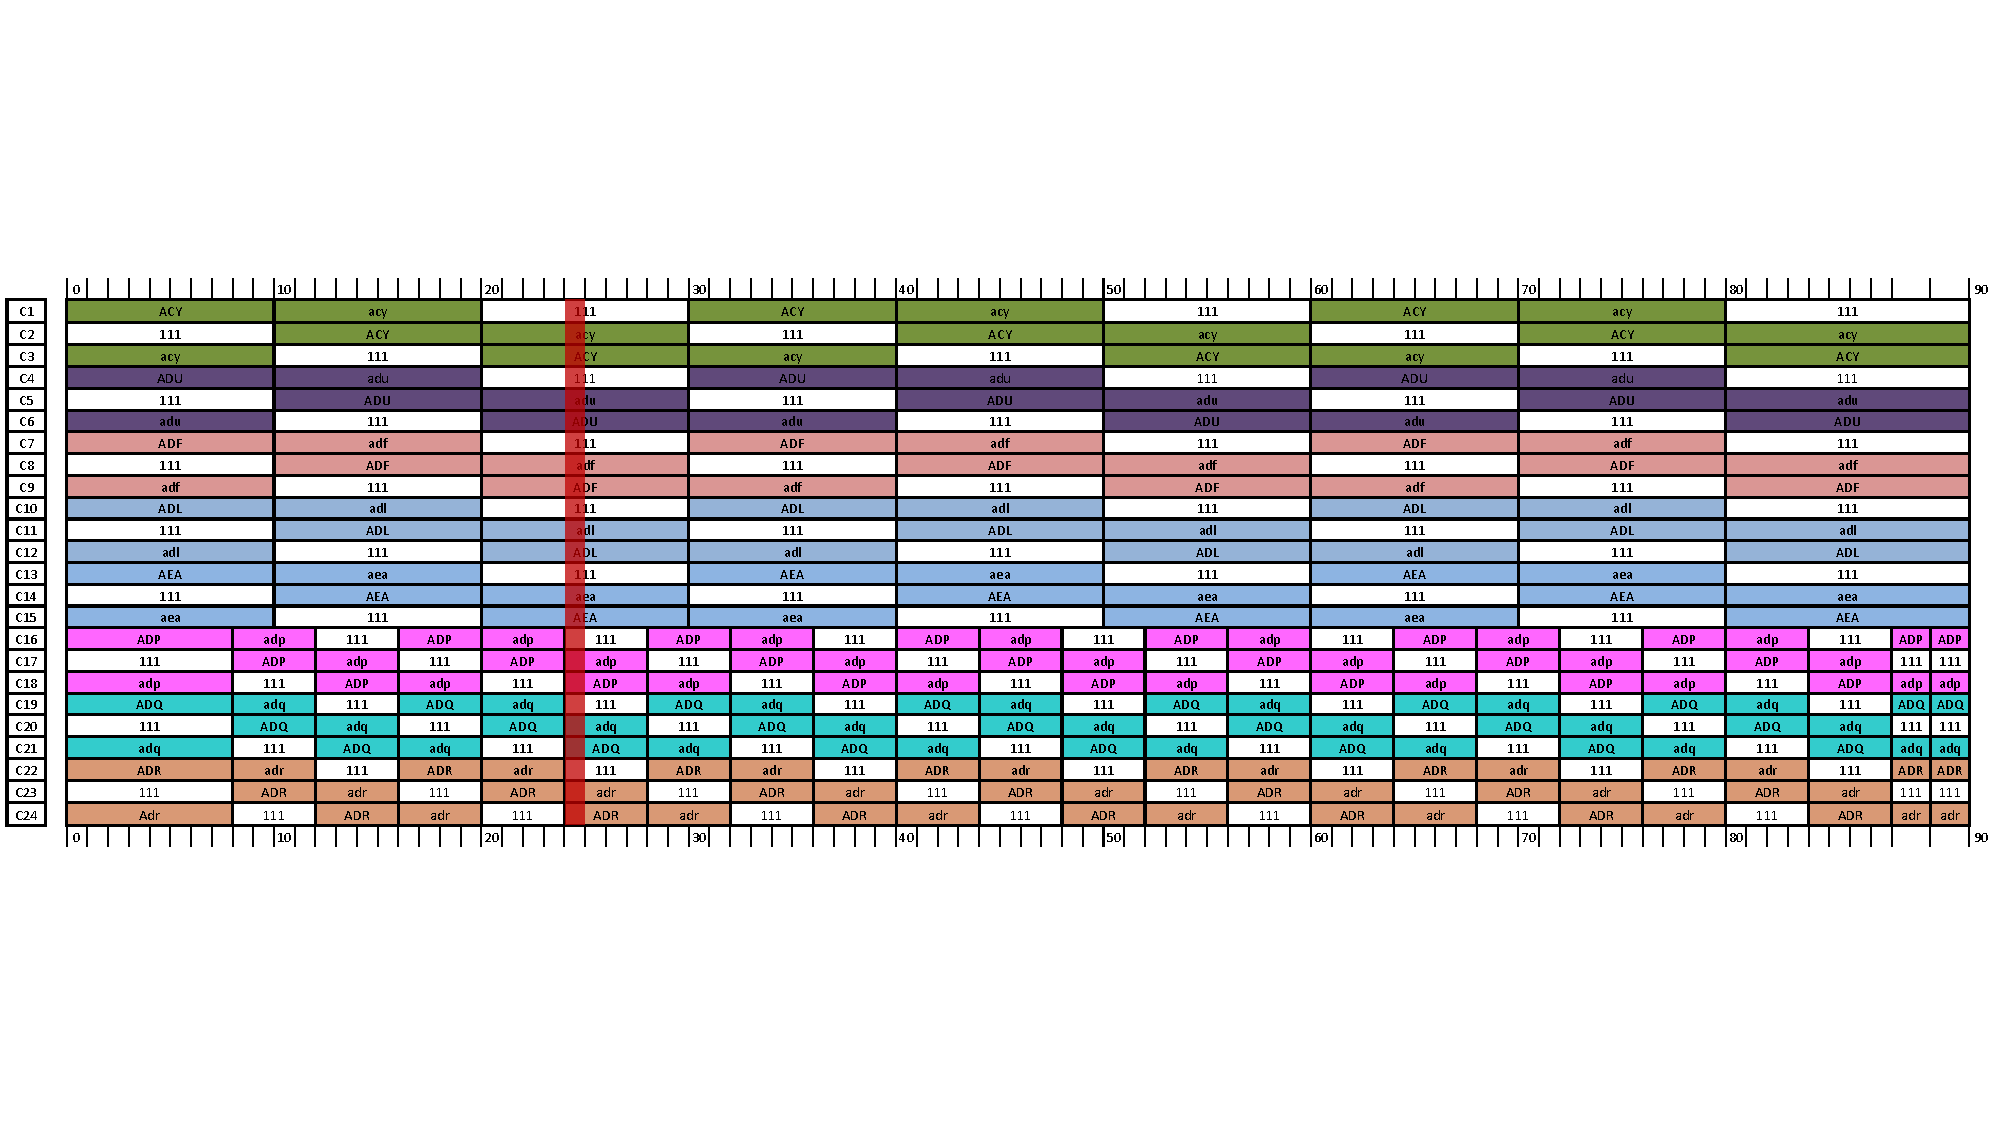
\includegraphics[width=\linewidth]{caso3/caso3-fase0}
	\caption{Planificación inicial del Caso 3}
	\label{fig:caso3-fase0}
\end{figure}

\begin{figure}[!h]
	\centering
	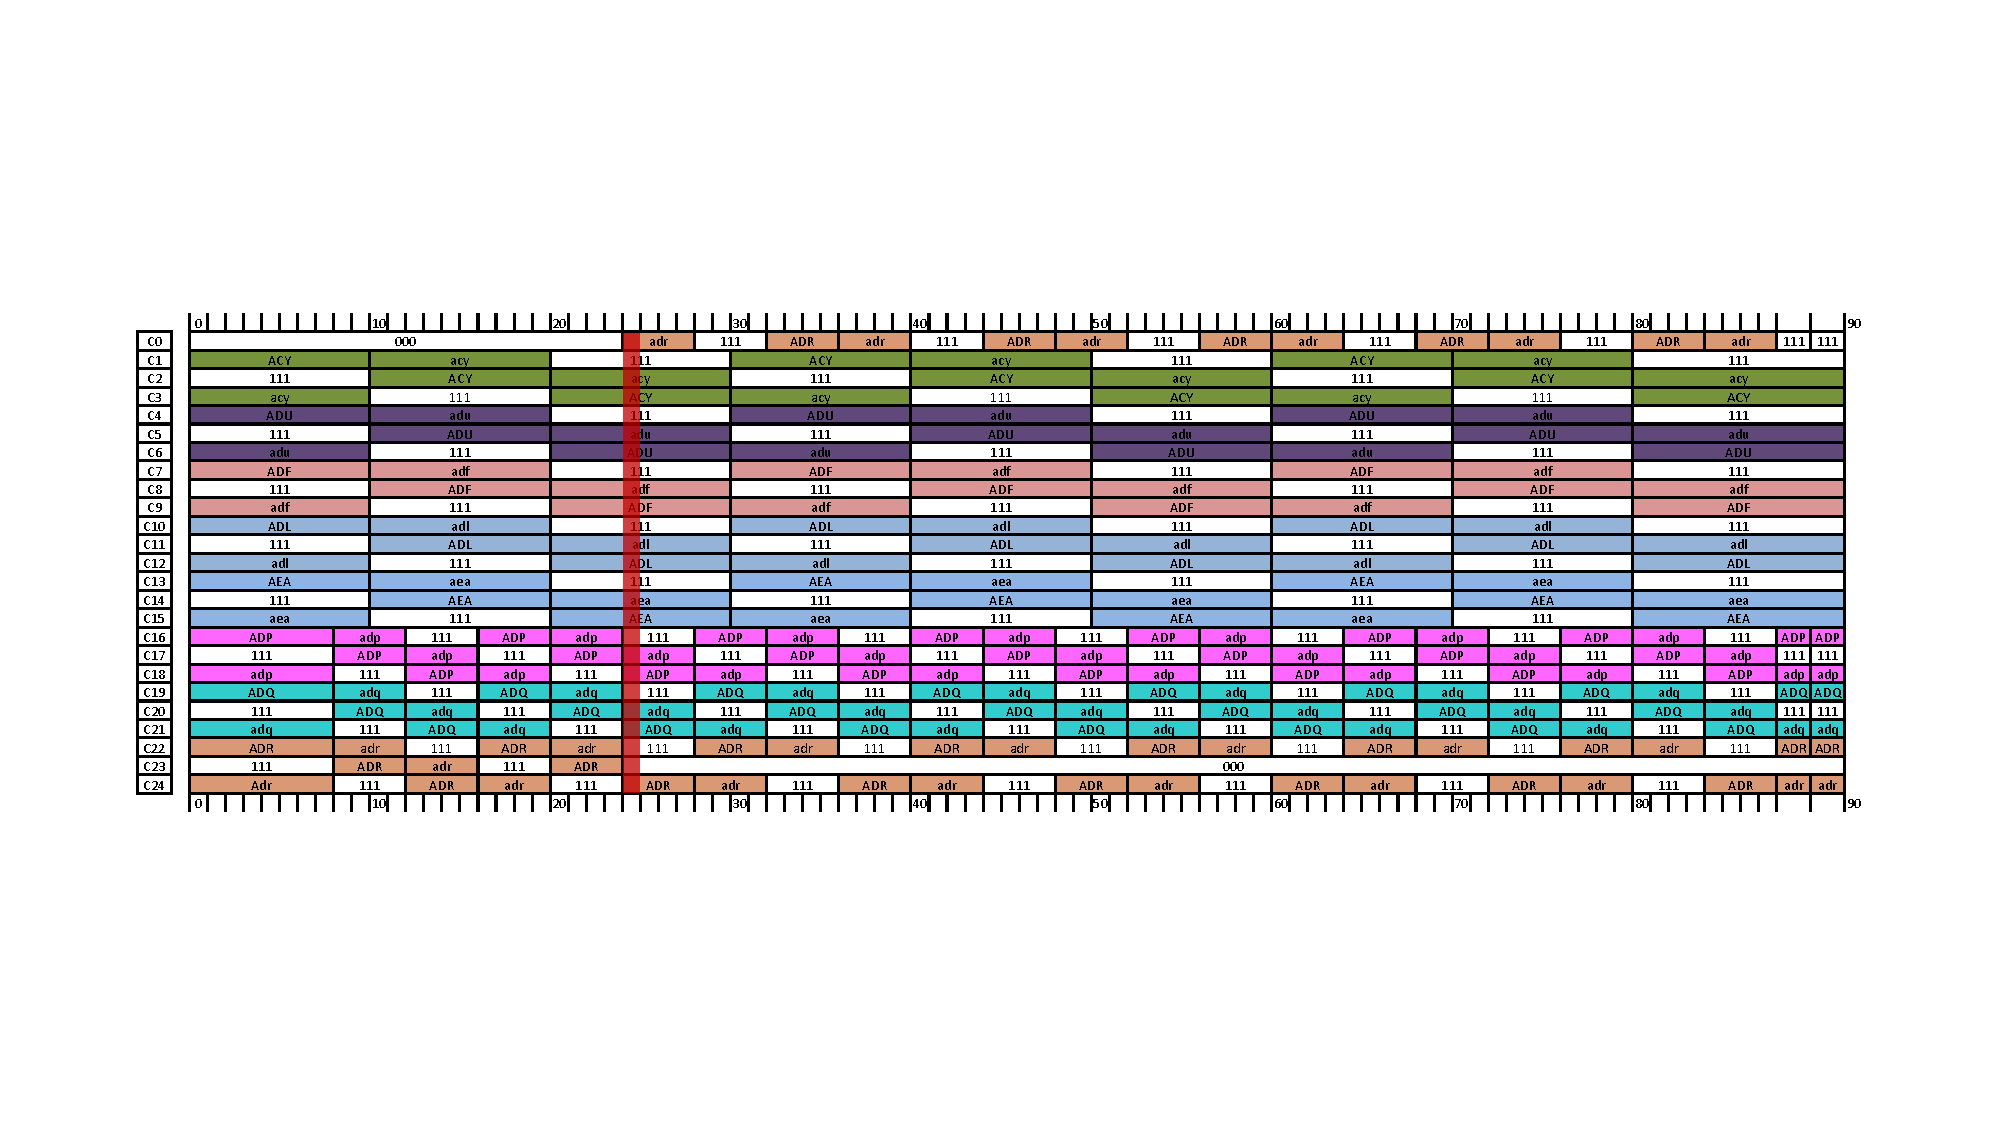
\includegraphics[width=\linewidth]{caso3/caso3-fase1}
	\caption{Solución inicial (\faseuno{}) para el Caso 3}
	\label{fig:caso3-fase1}
\end{figure}

\begin{figure}[!h]
	\centering
	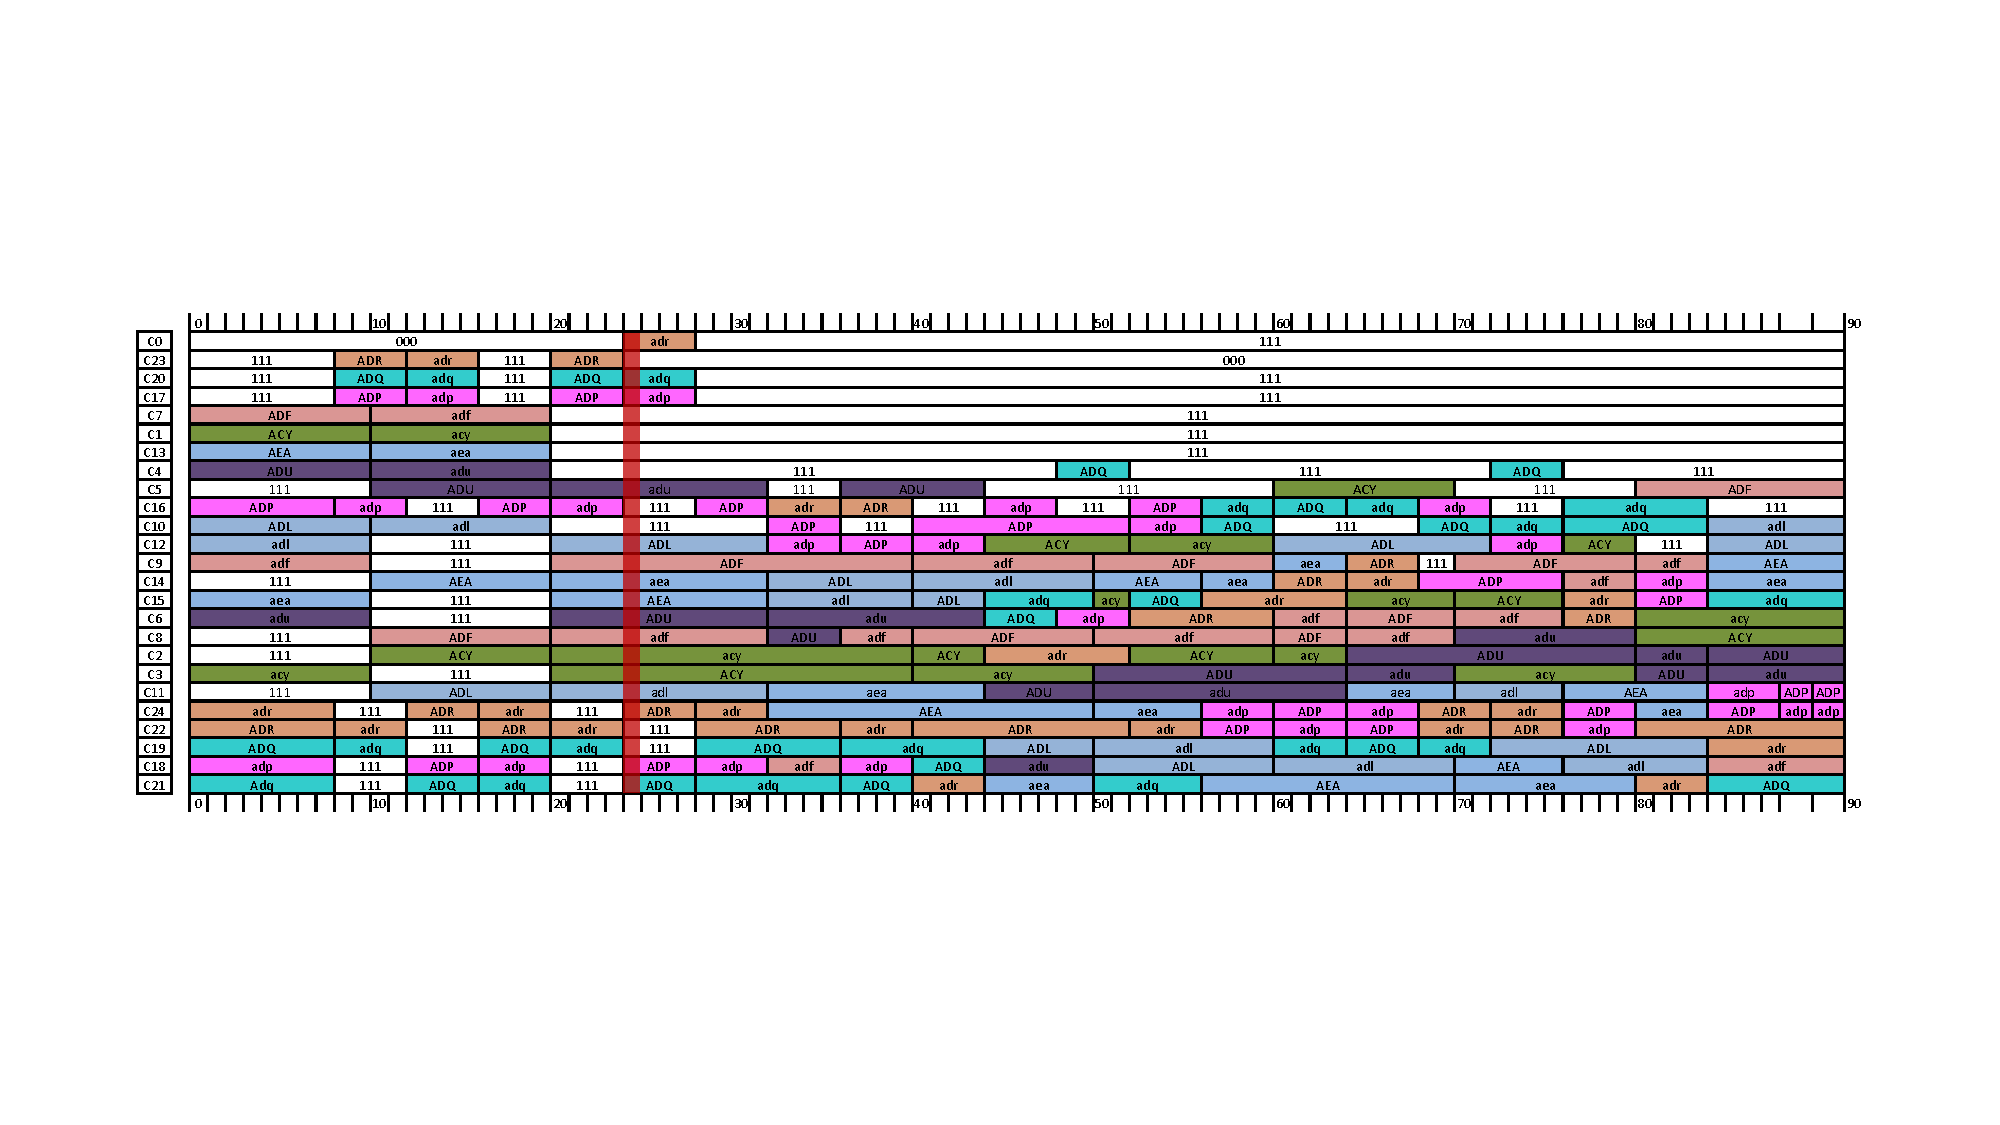
\includegraphics[width=\linewidth]{caso3/caso3-fase2}
	\caption{Solución final (\fasedos{}) para el Caso 3}
	\label{fig:caso3-fase2}
\end{figure}

\FloatBarrier
\newpage
\subsection{Caso 4}

\begin{figure}[!h]
	\centering
	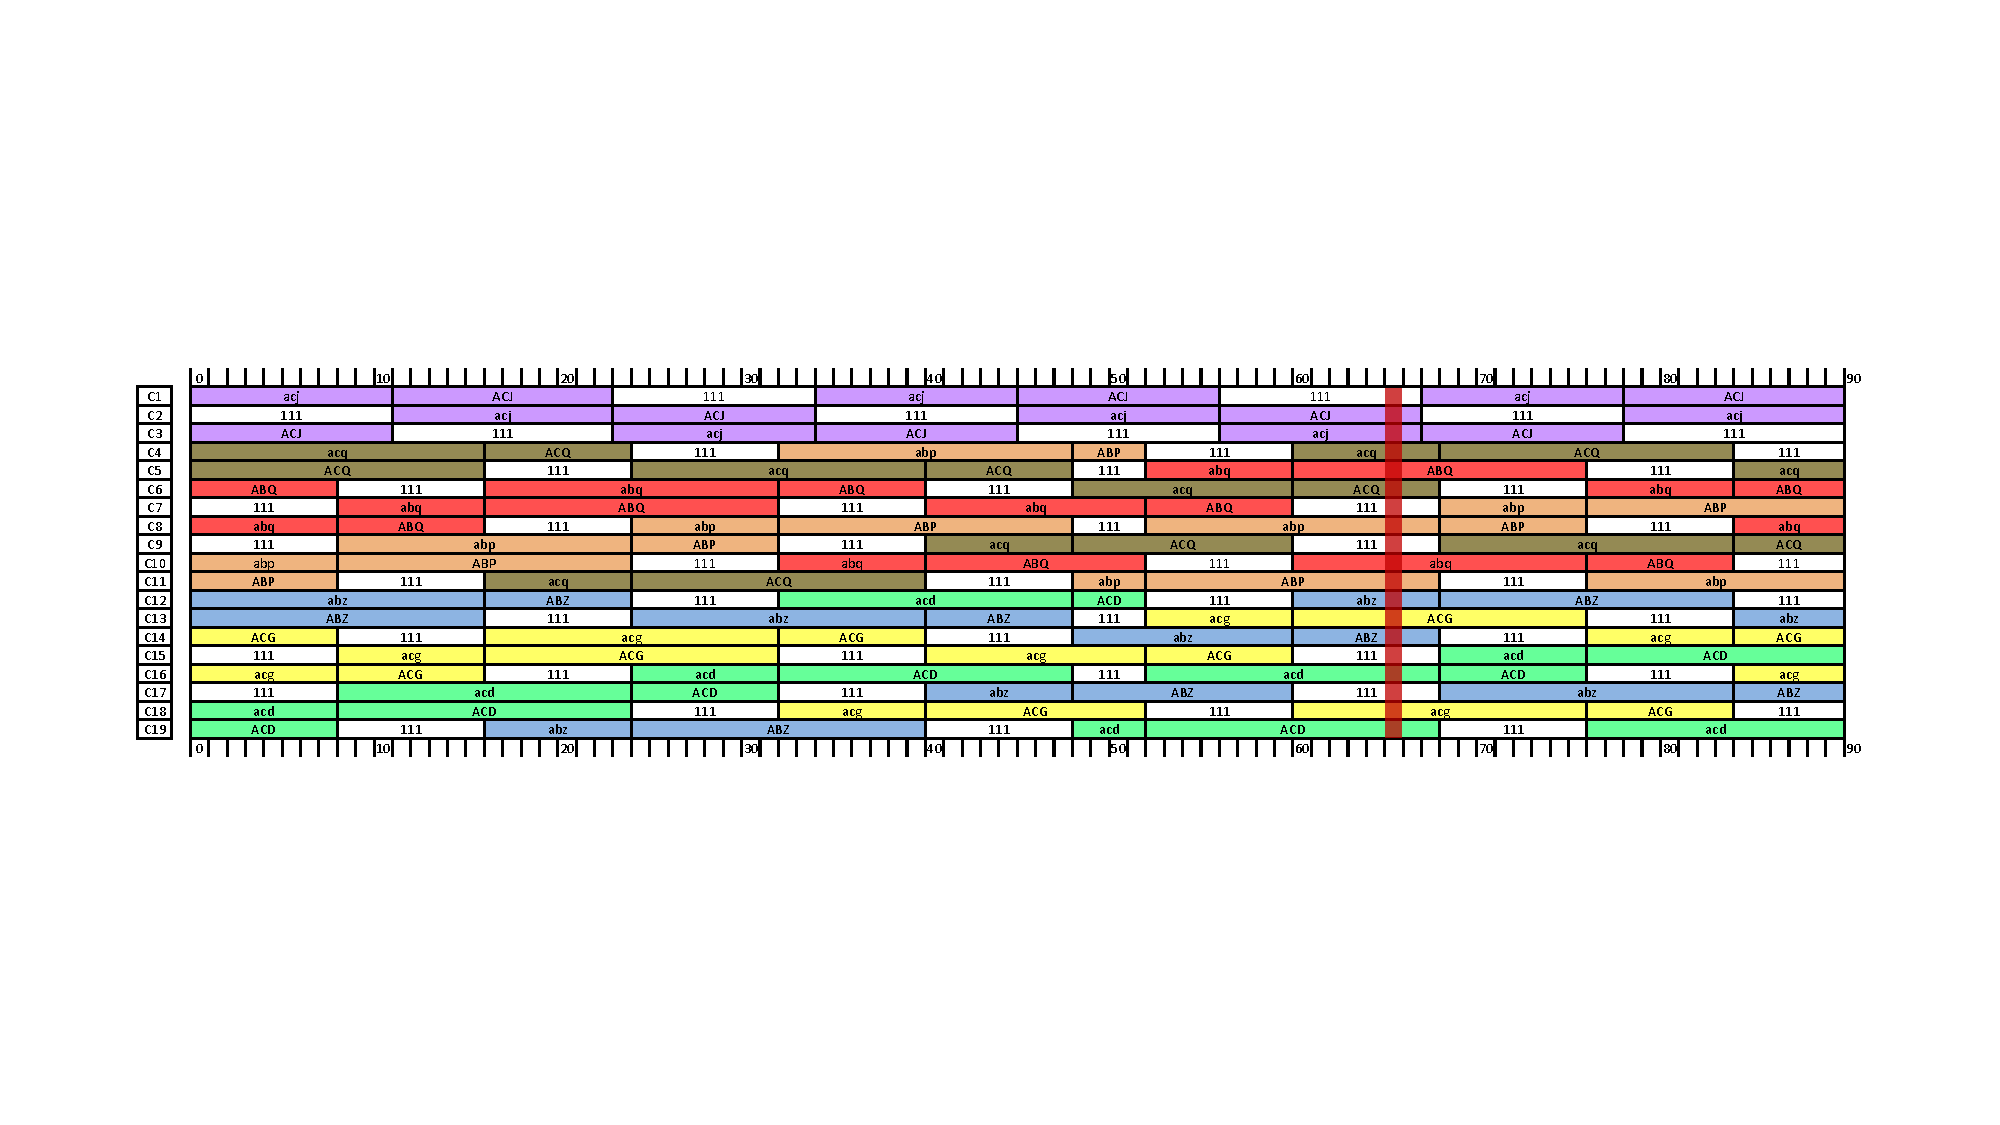
\includegraphics[width=\linewidth]{caso4/caso4-fase0}
	\caption{Planificación inicial del Caso 4}
	\label{fig:caso4-fase0}
\end{figure}

\begin{figure}[!h]
	\centering
	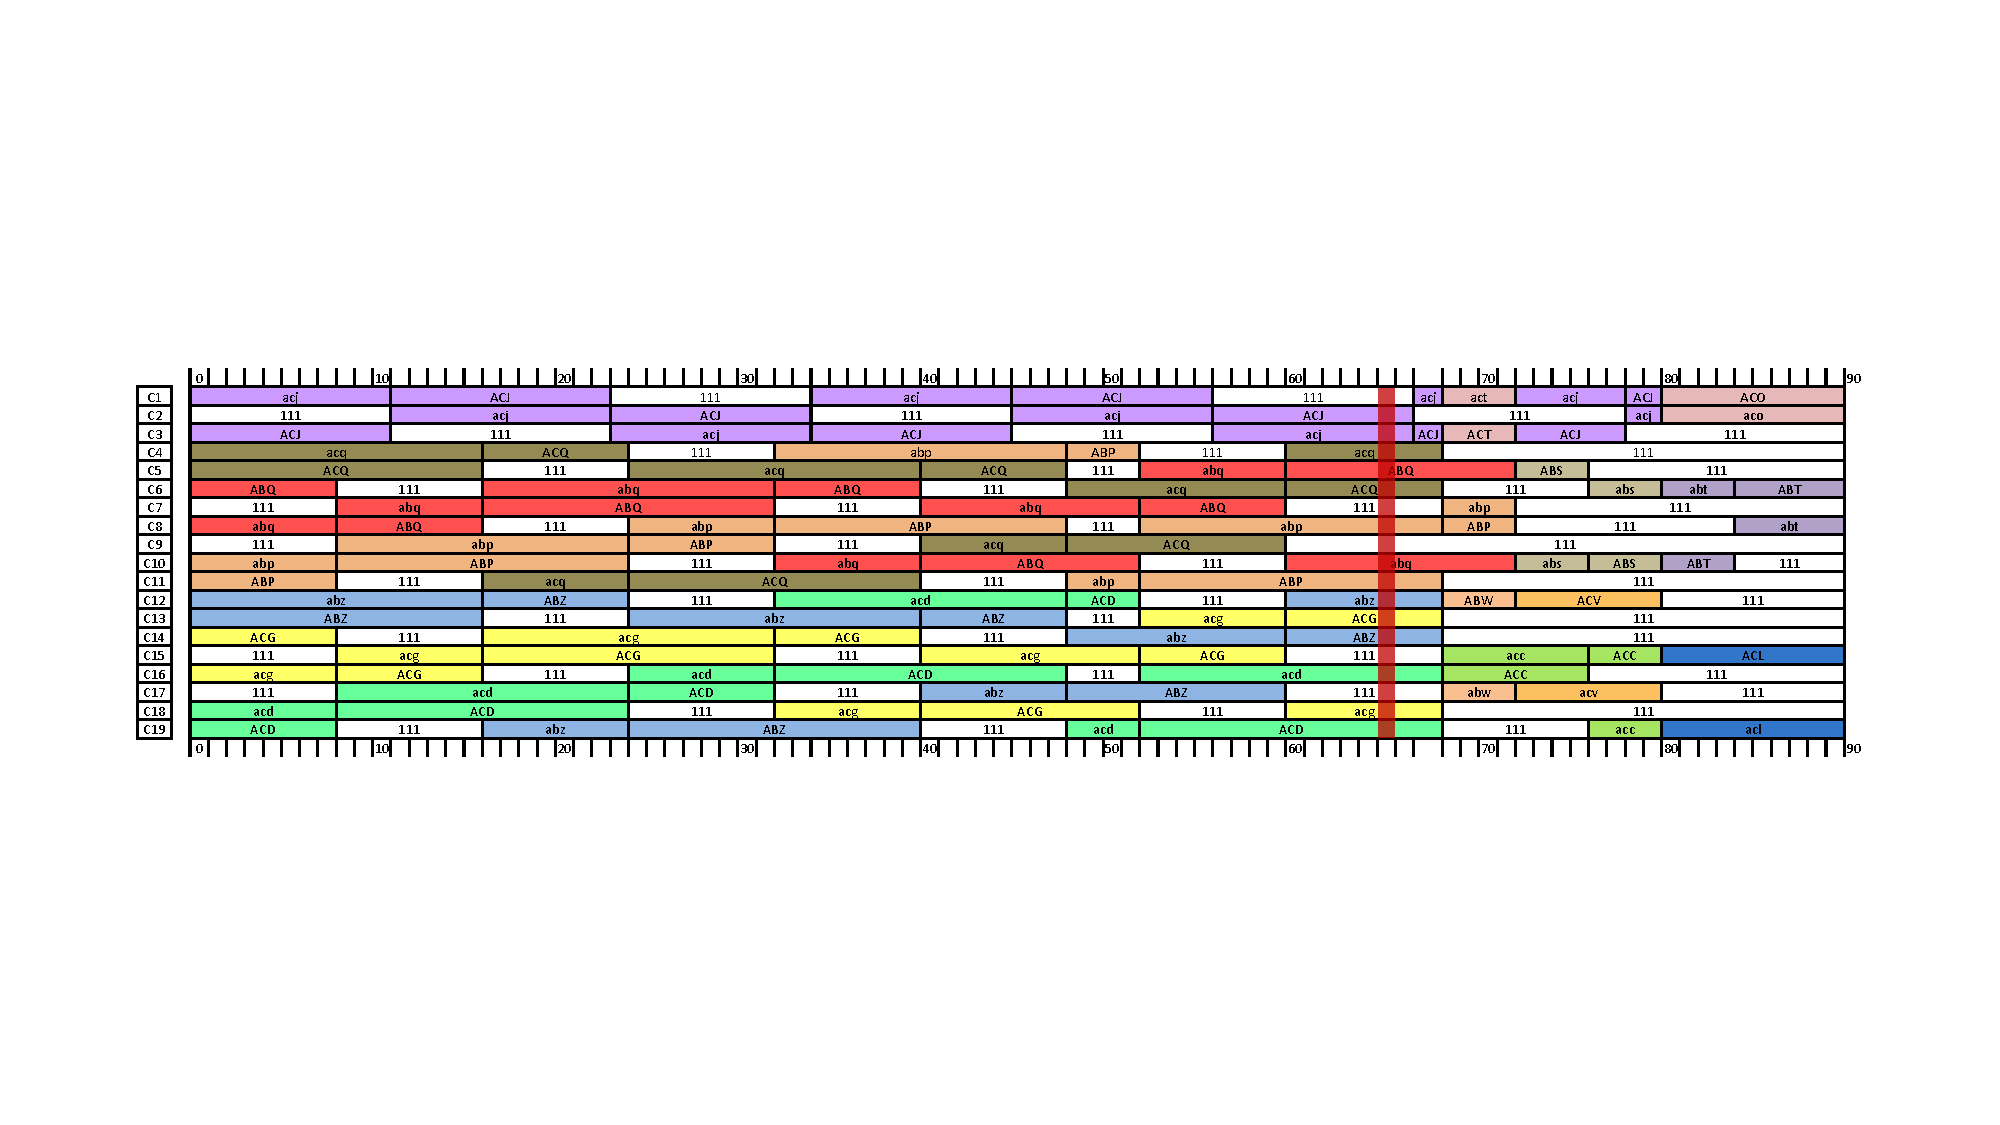
\includegraphics[width=\linewidth]{caso4/caso4-fase1}
	\caption{Solución inicial (\faseuno{}) para el Caso 4}
	\label{fig:caso4-fase1}
\end{figure}

\begin{figure}[!h]
	\centering
	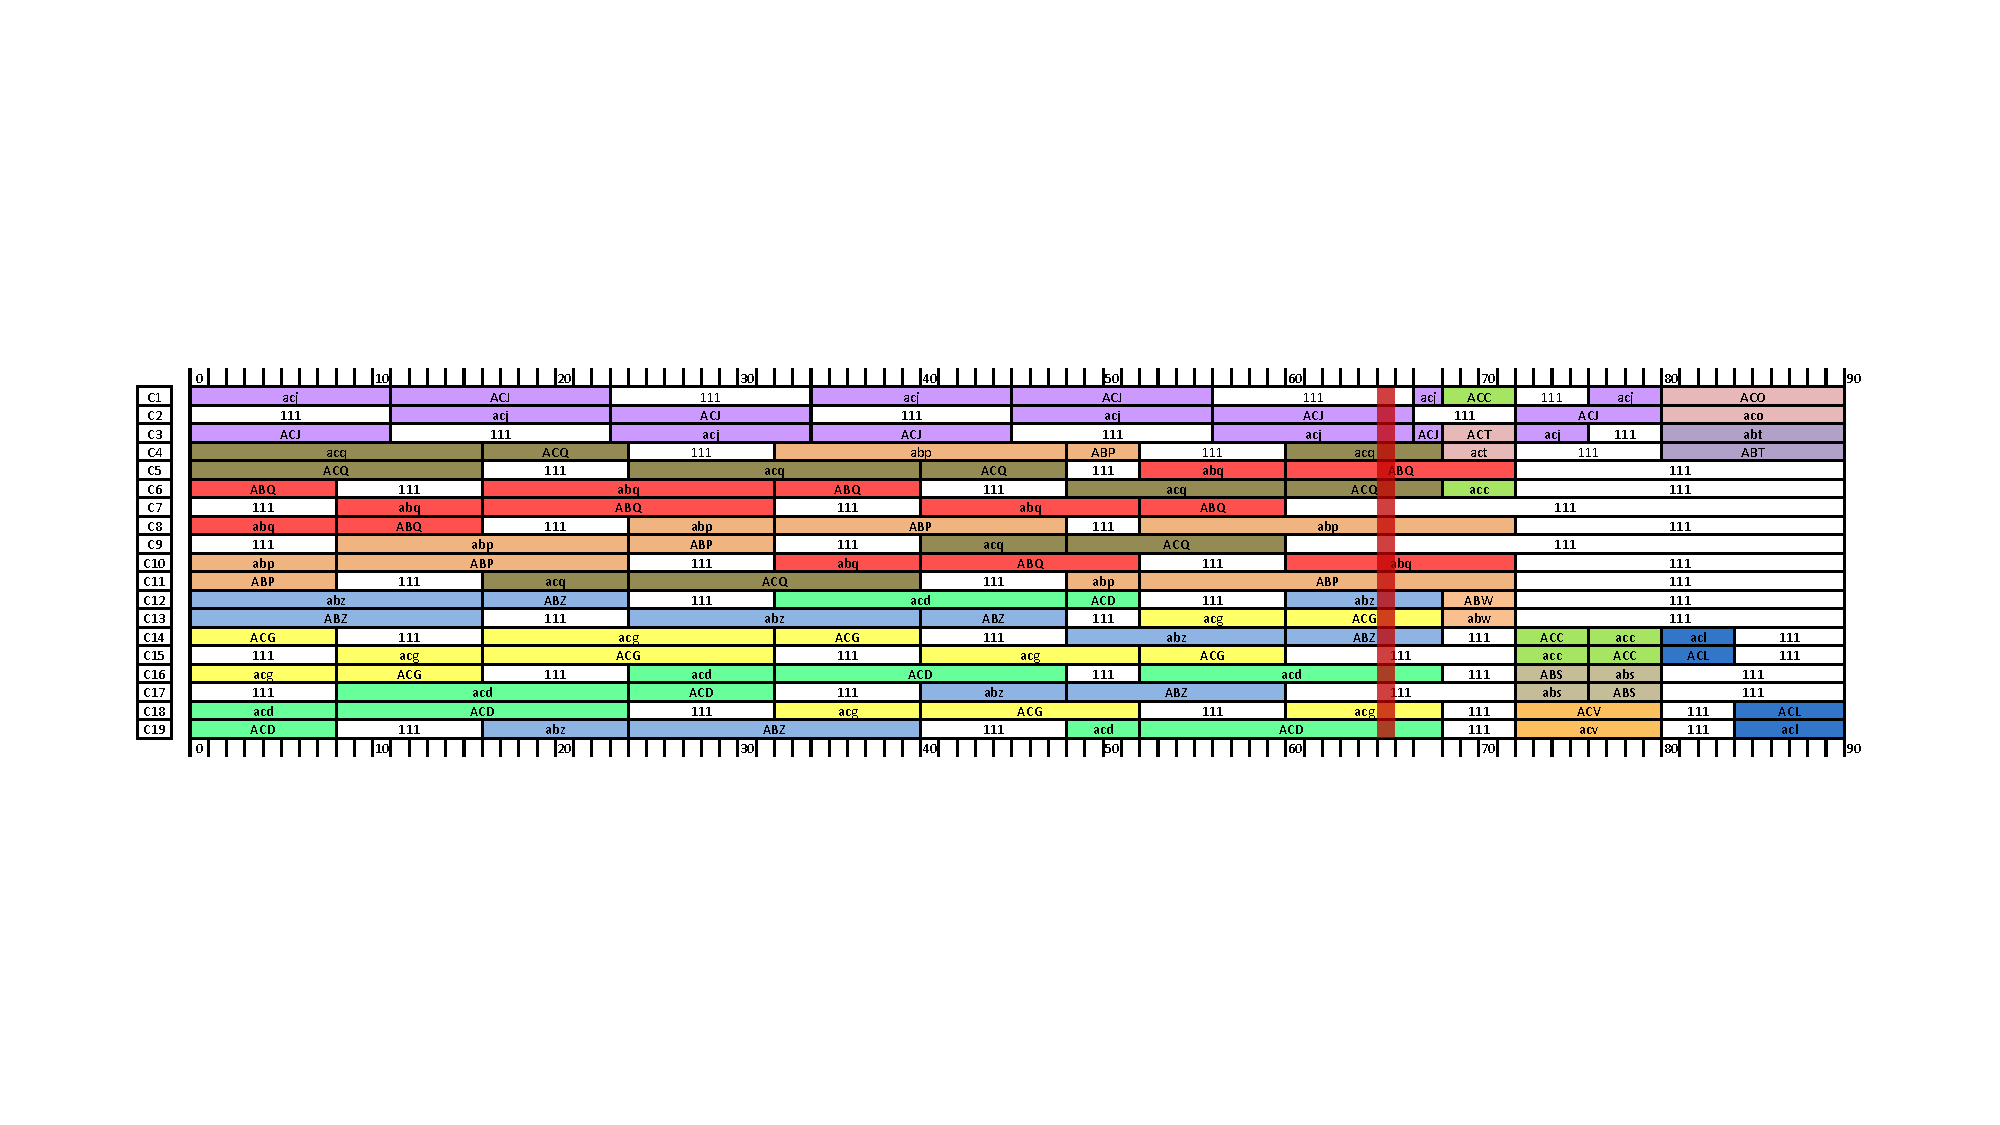
\includegraphics[width=\linewidth]{caso4/caso4-fase2}
	\caption{Solución final (\fasedos{}) para el Caso 4}
	\label{fig:caso4-fase2}
\end{figure}

\FloatBarrier
\newpage
\subsection{Caso 5}

La planificación inicial es la misma que la del Caso 4, cambiando el slot del momento del cambio.

\begin{figure}[!h]
	\centering
	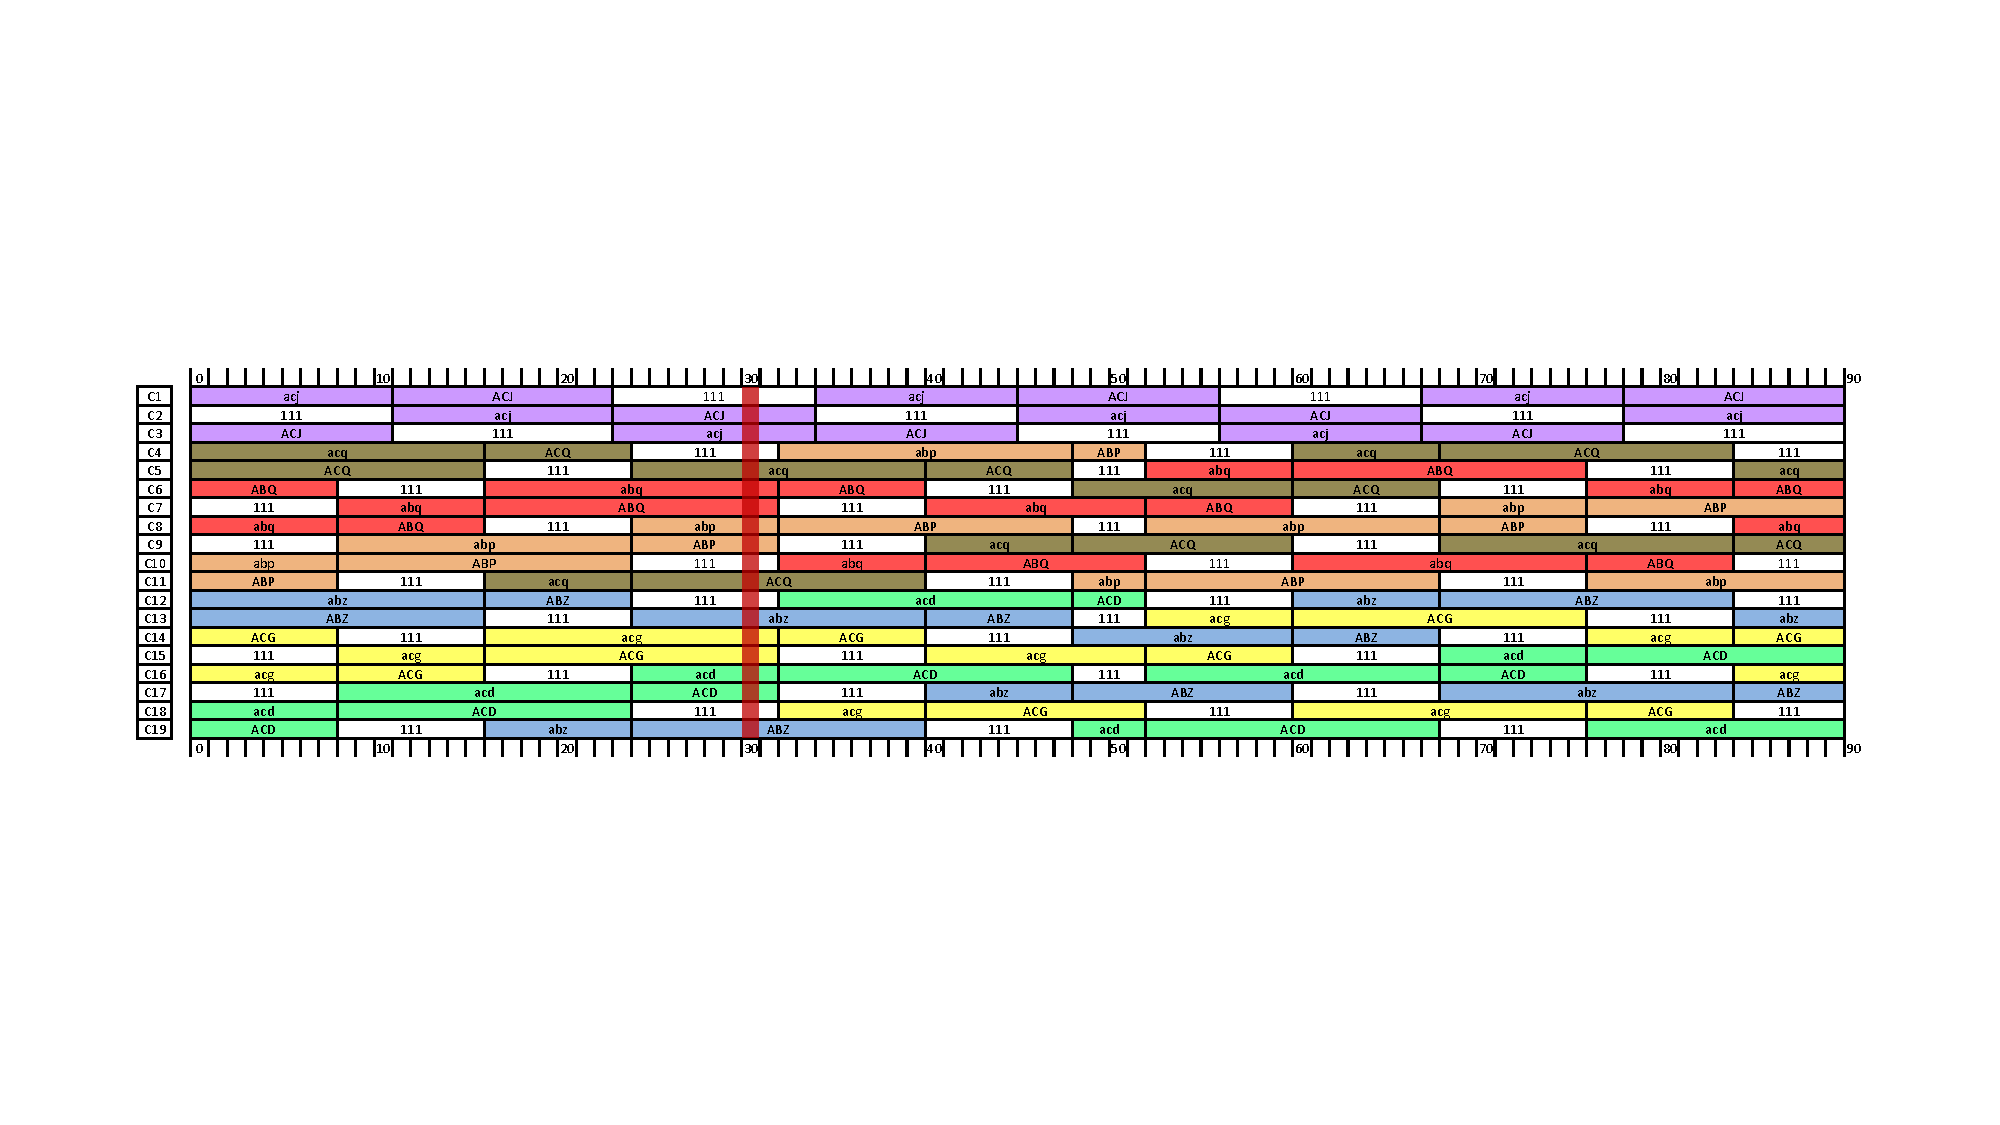
\includegraphics[width=\linewidth]{caso5/caso5-fase0}
	\caption{Planificación inicial del Caso 5}
	\label{fig:caso5-fase0}
\end{figure}

\begin{figure}[!h]
	\centering
	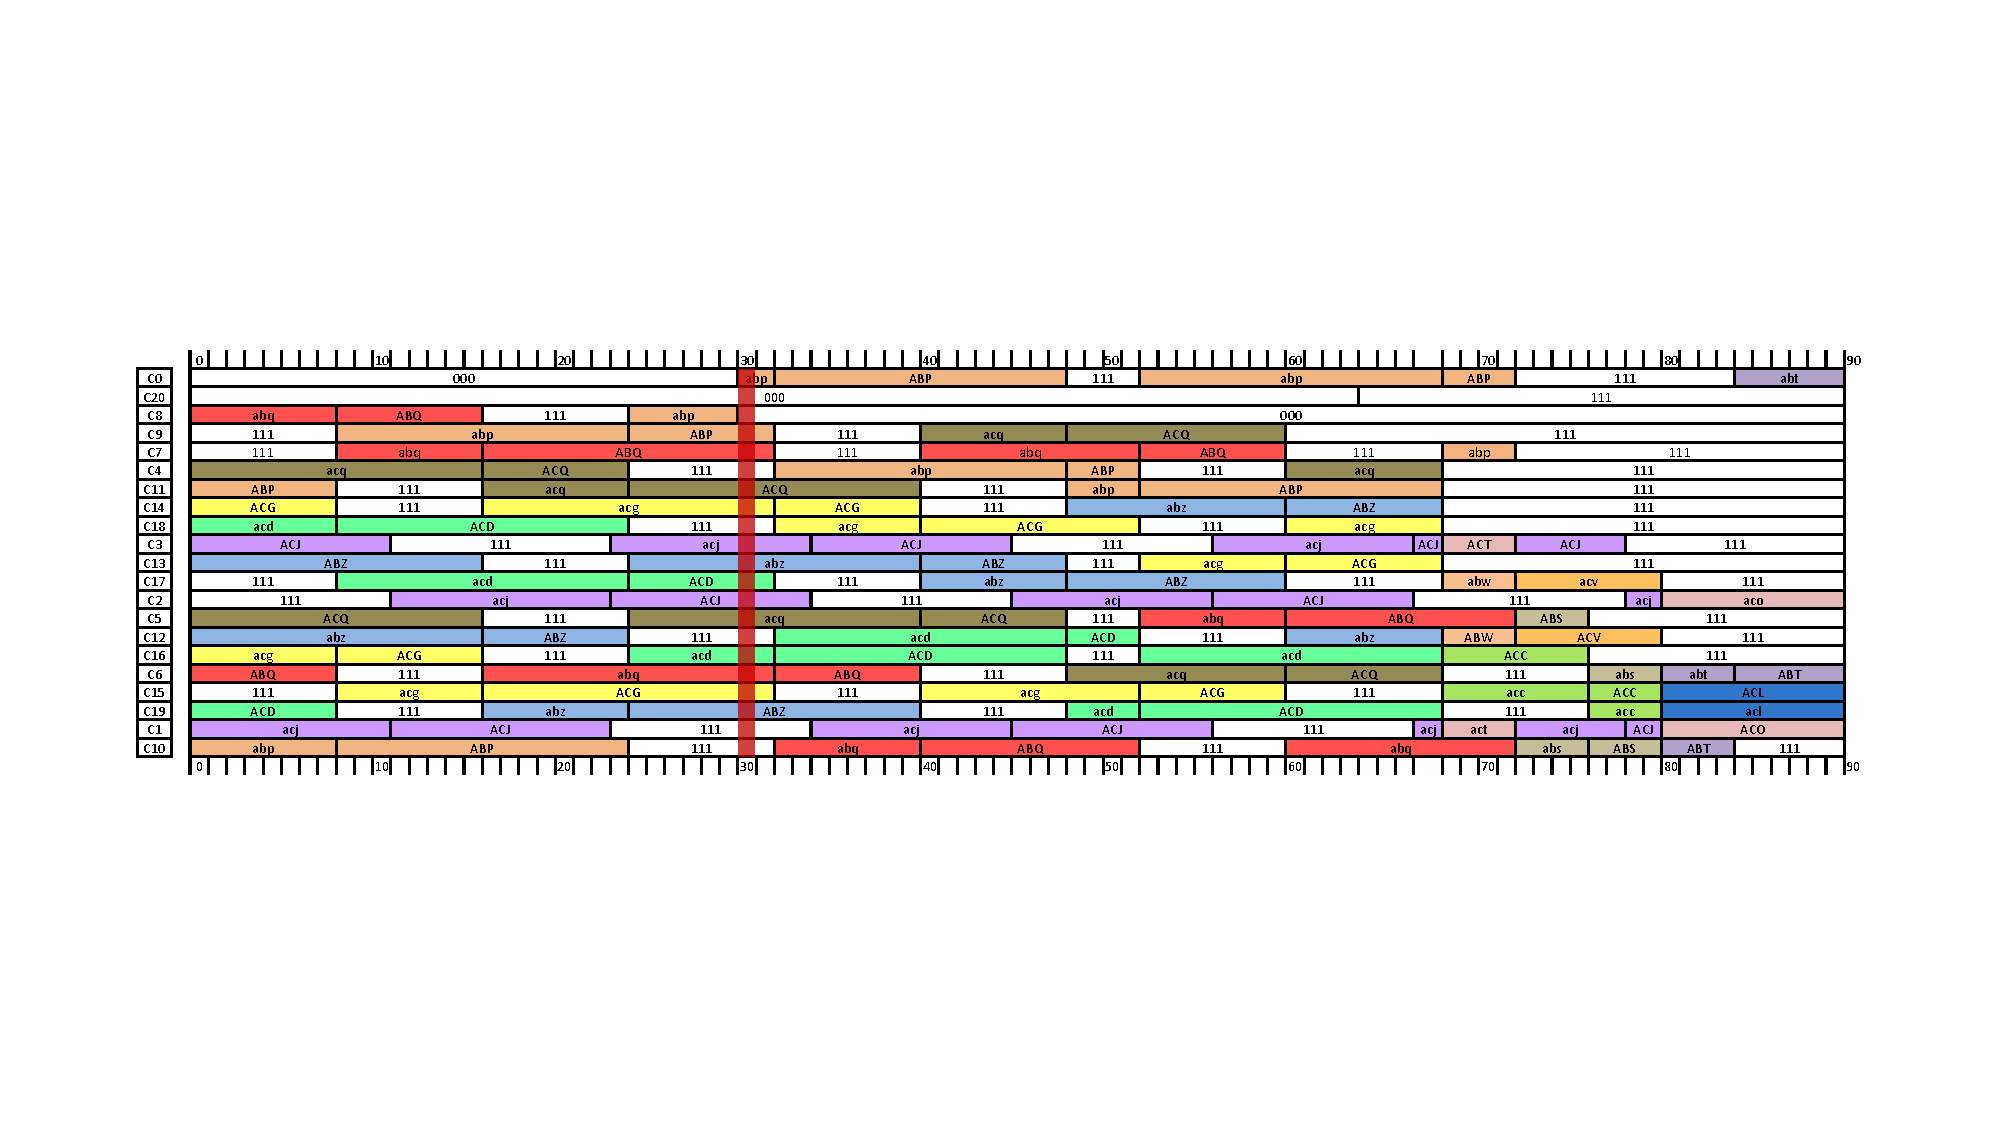
\includegraphics[width=\linewidth]{caso5/caso5-fase1}
	\caption{Solución inicial (\faseuno{}) para el Caso 5}
	\label{fig:caso5-fase1}
\end{figure}

\begin{figure}[!h]
	\centering
	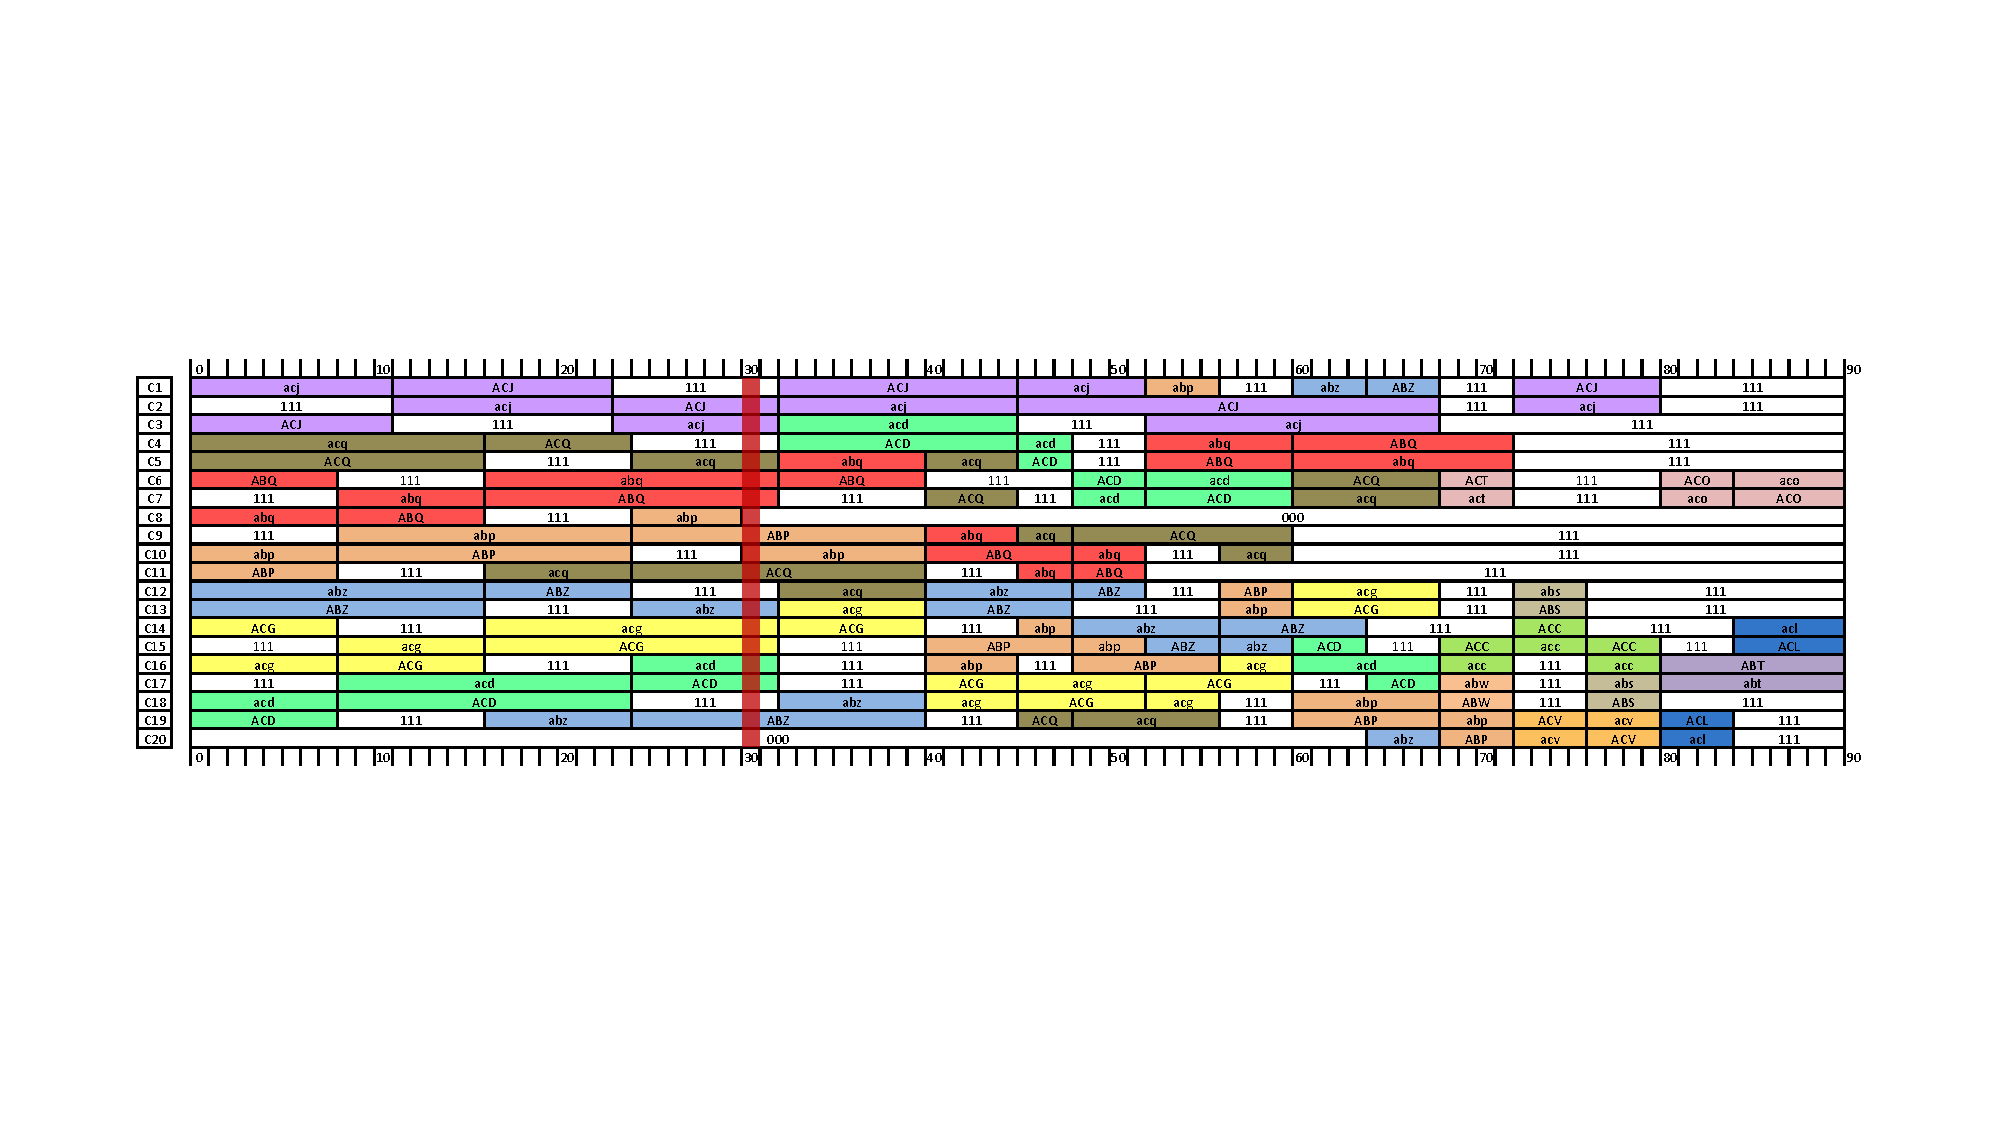
\includegraphics[width=\linewidth]{caso5/caso5-fase2}
	\caption{Solución final (\fasedos{}) para el Caso 5}
	\label{fig:caso5-fase2}
\end{figure}

\FloatBarrier
\newpage
\subsection{Caso 6}

La planificación inicial es la misma que la del Caso 4, cambiando el slot del momento del cambio.

\begin{figure}[!h]
	\centering
	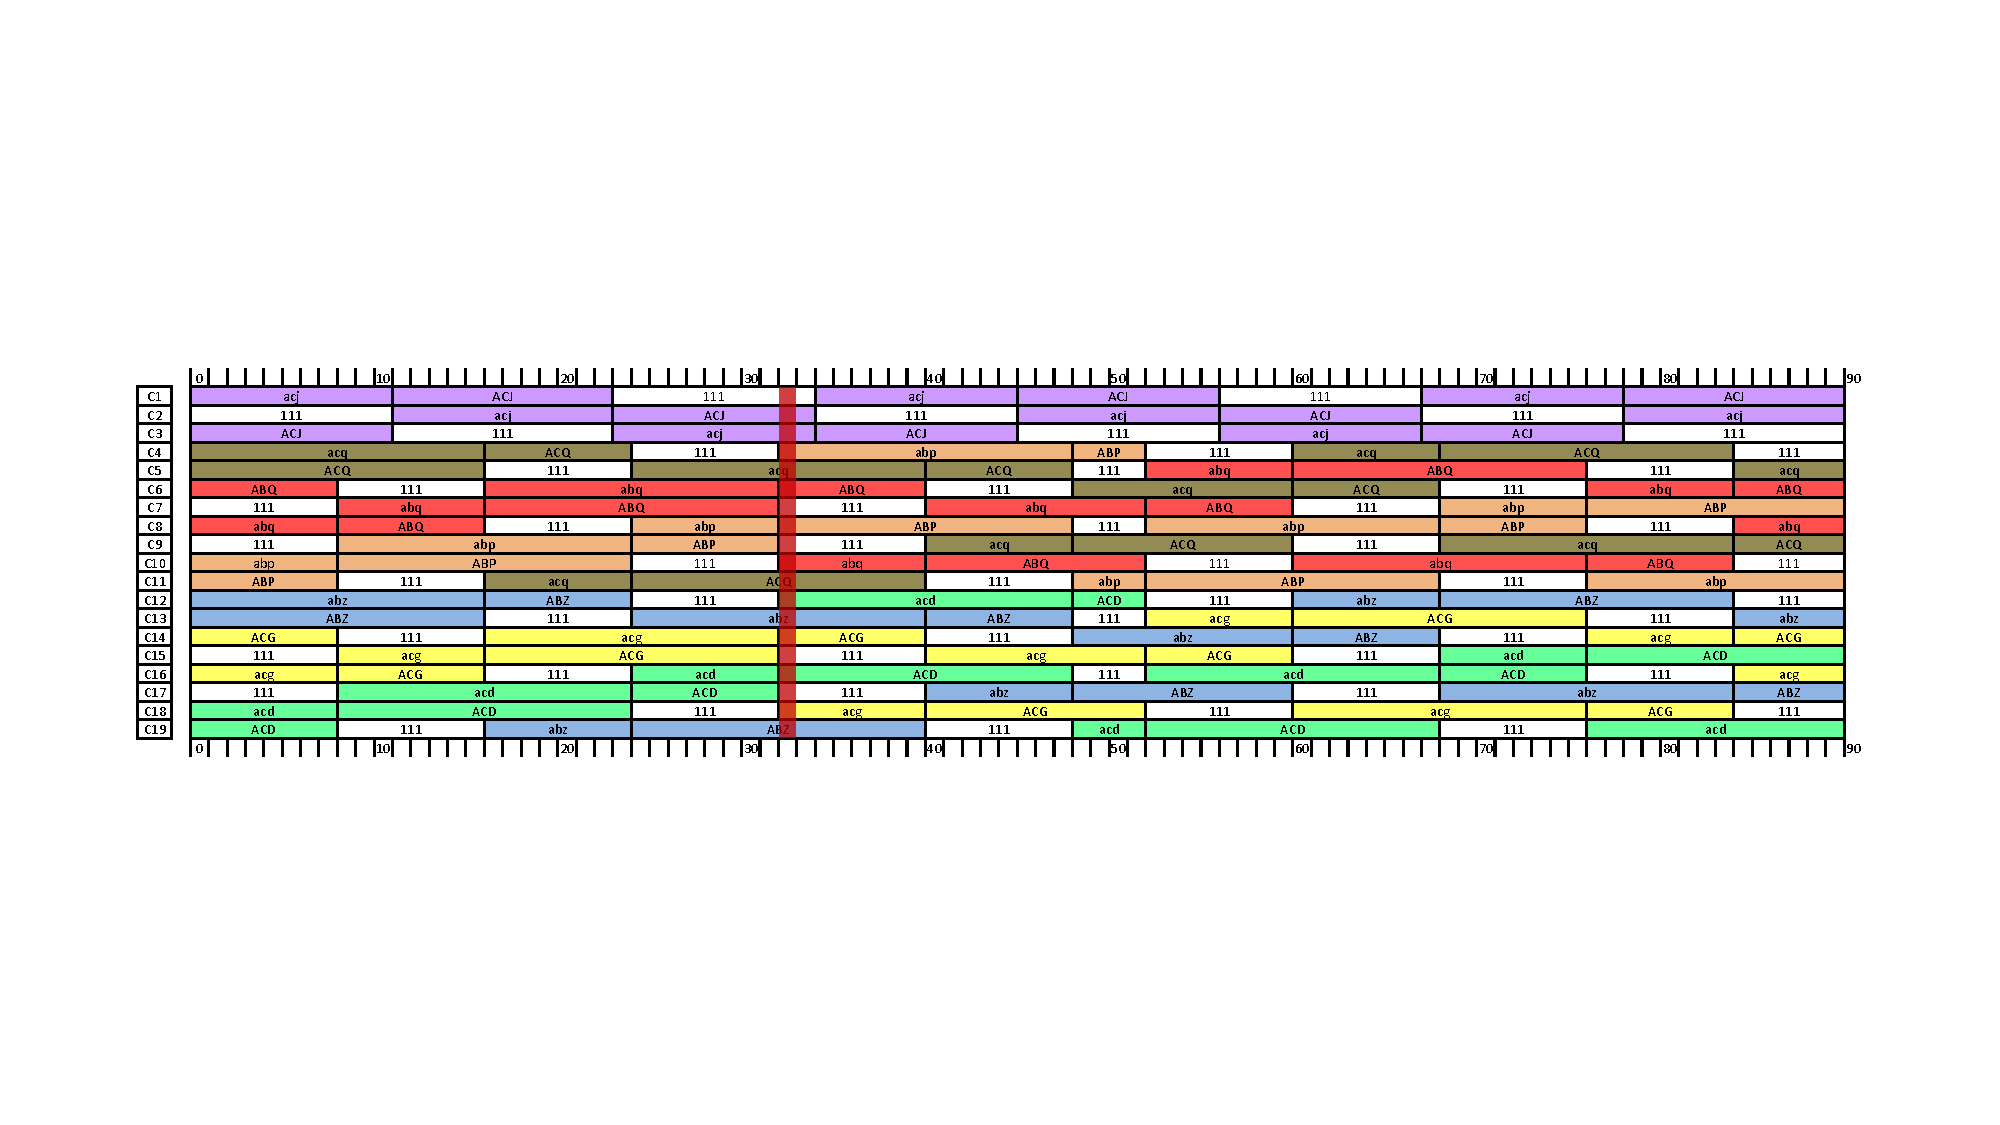
\includegraphics[width=\linewidth]{caso6/caso6-fase0}
	\caption{Planificación inicial del Caso 6}
	\label{fig:caso6-fase0}
\end{figure}

\begin{figure}[!h]
	\centering
	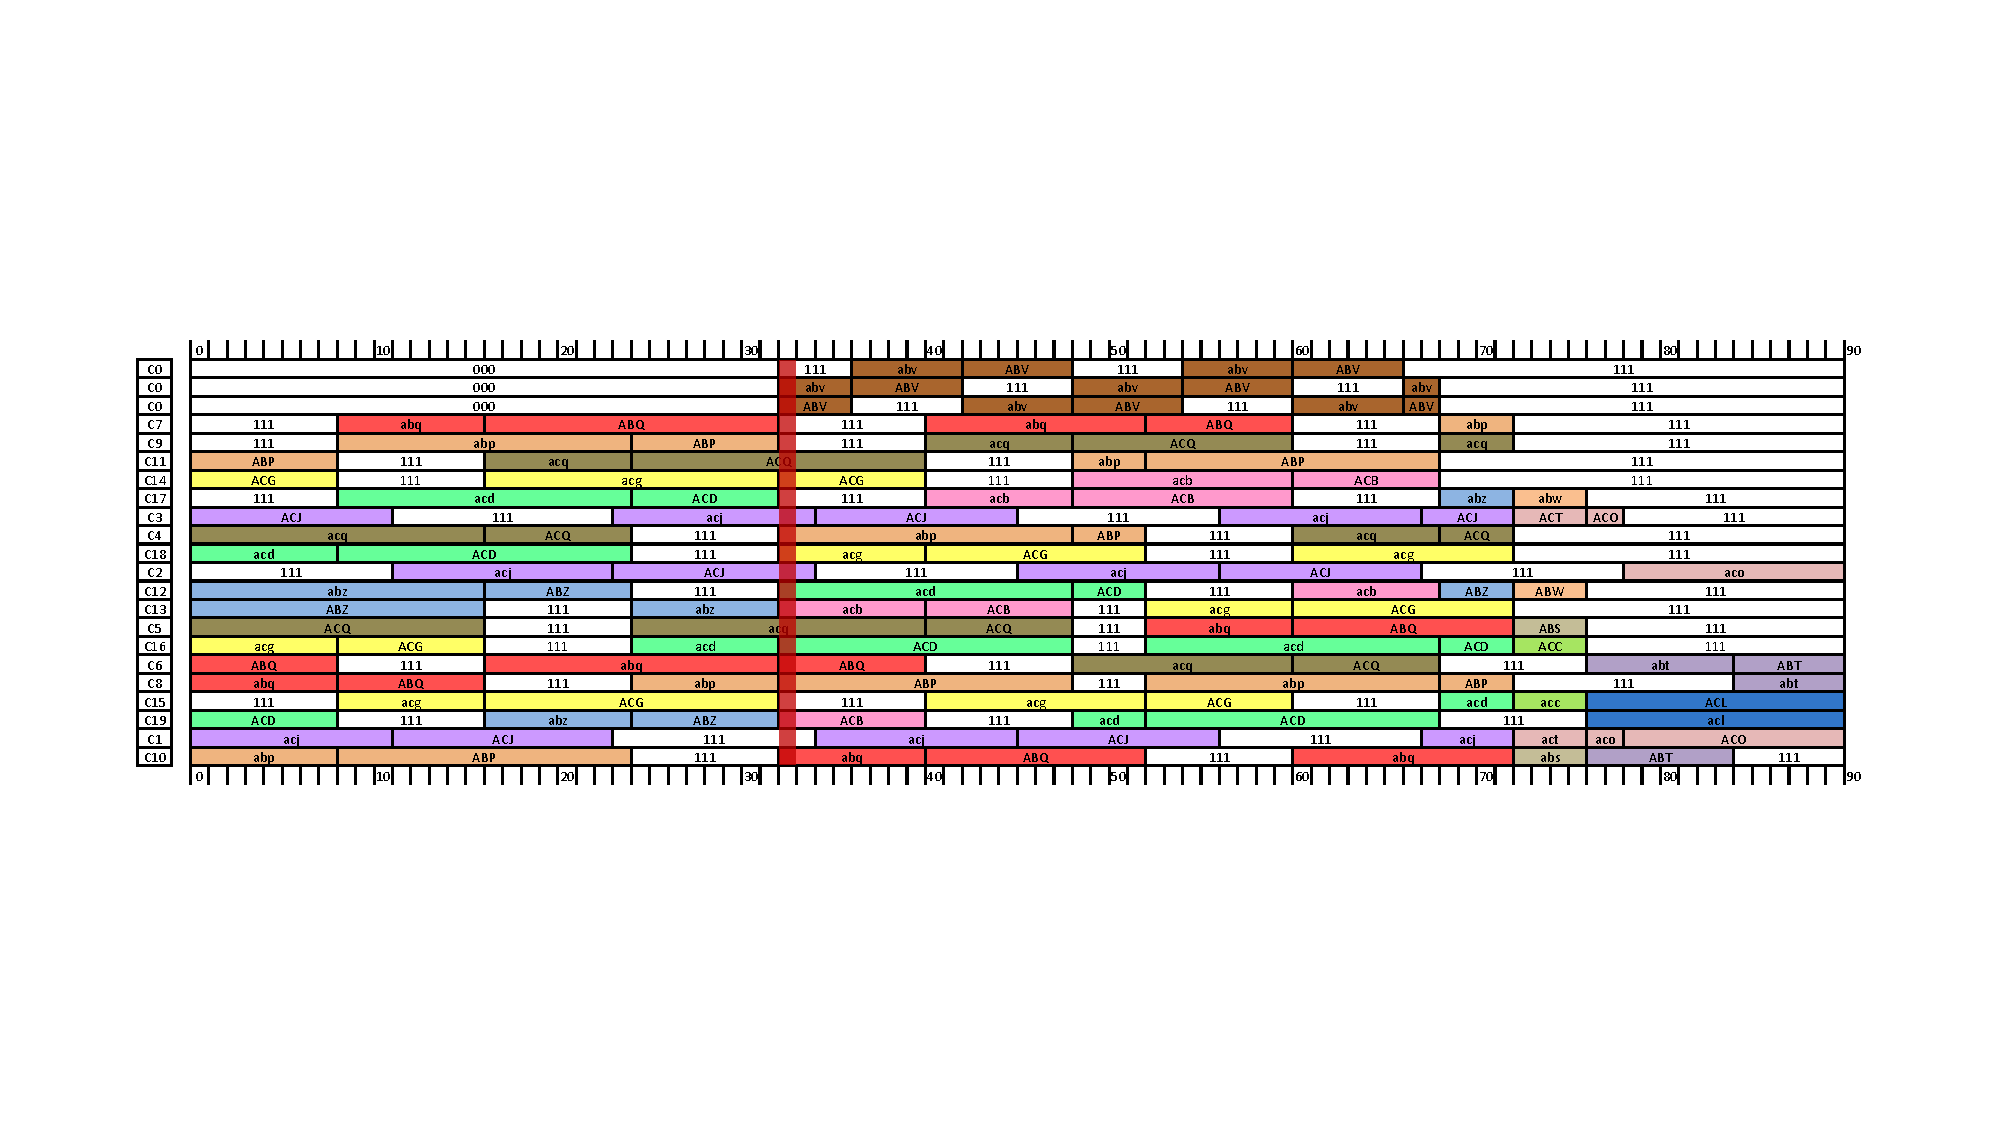
\includegraphics[width=\linewidth]{caso6/caso6-fase1}
	\caption{Solución inicial (\faseuno{}) para el Caso 6}
	\label{fig:caso6-fase1}
\end{figure}

\begin{figure}[!h]
	\centering
	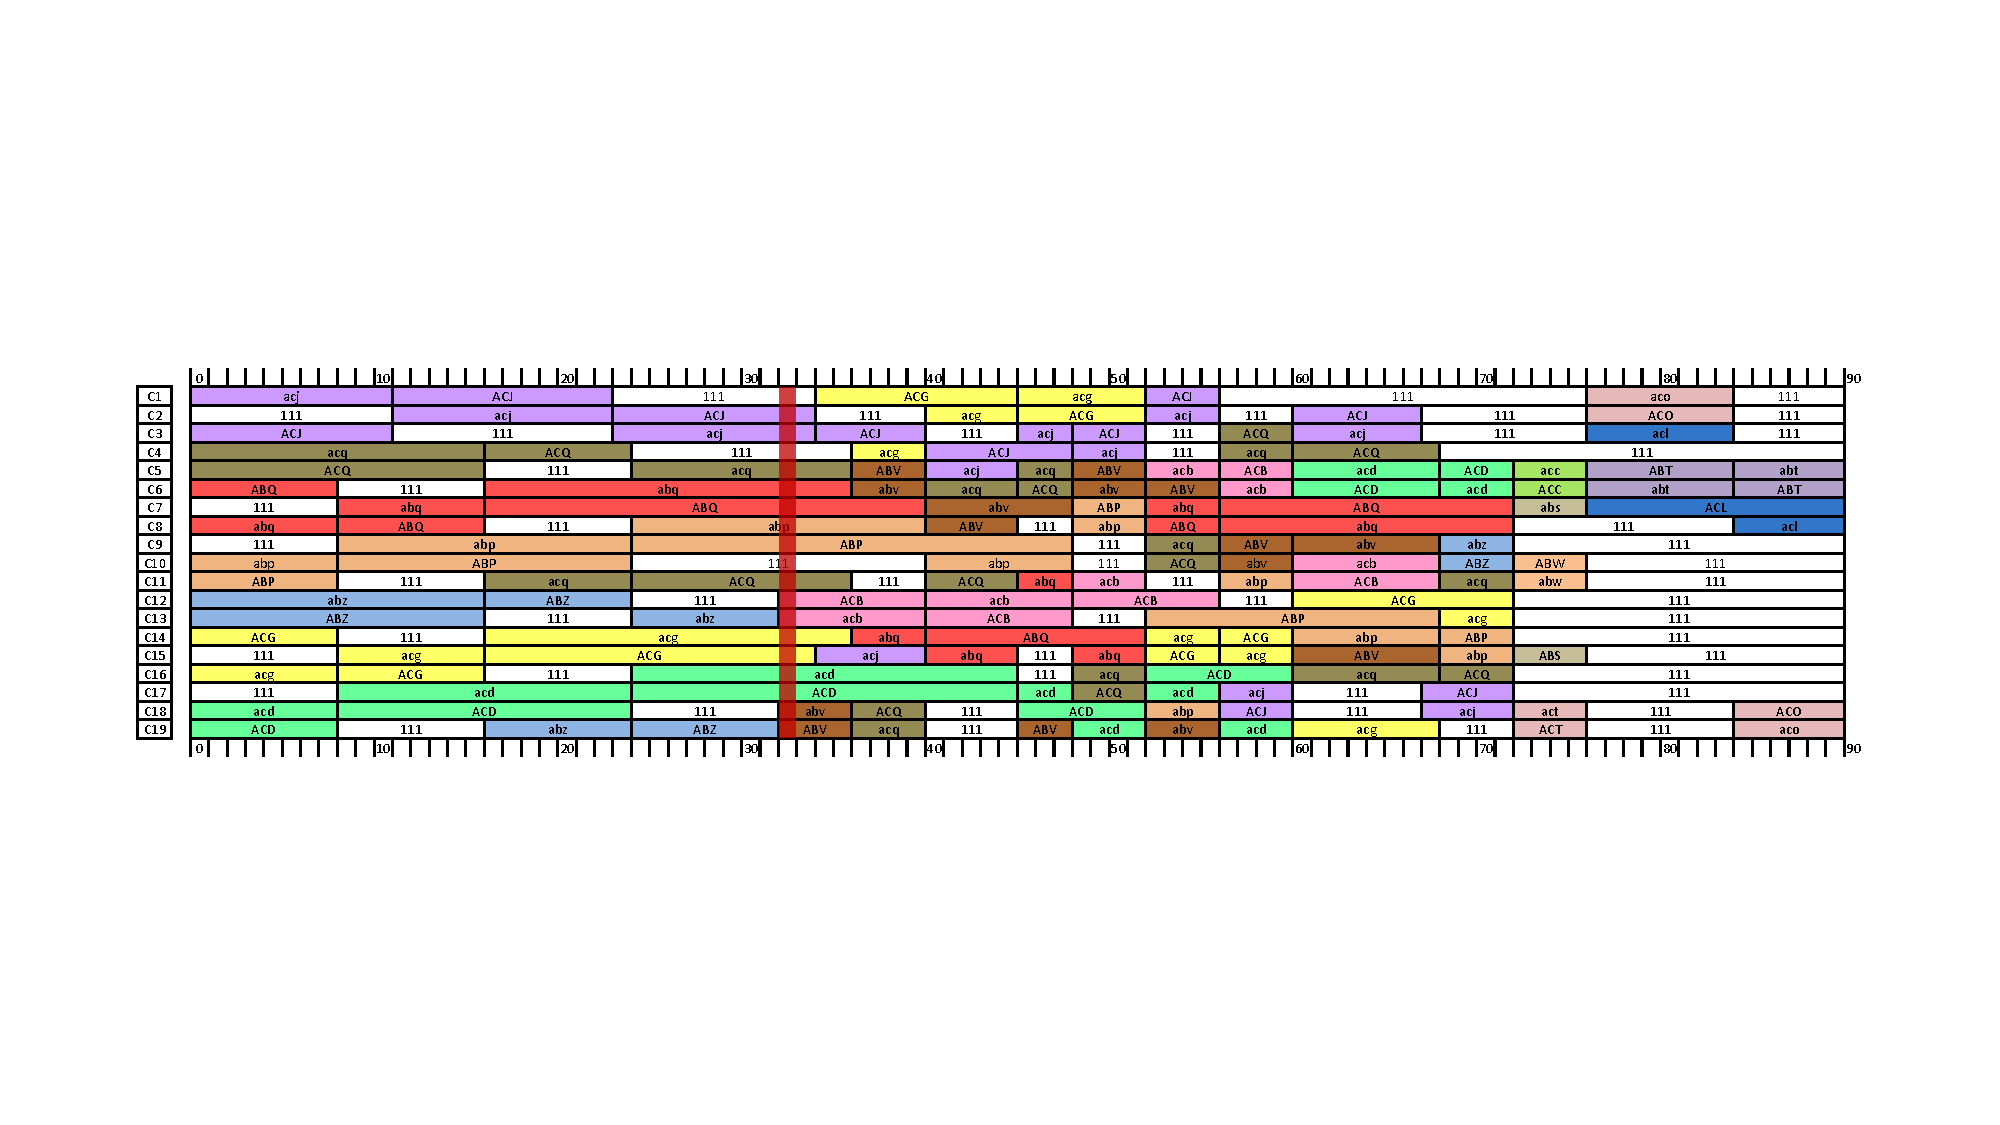
\includegraphics[width=\linewidth]{caso6/caso6-fase2}
	\caption{Solución final (\fasedos{}) para el Caso 6}
	\label{fig:caso6-fase2}
\end{figure}

\FloatBarrier
\newpage
\subsection{Caso 7}

\begin{figure}[!h]
	\centering
	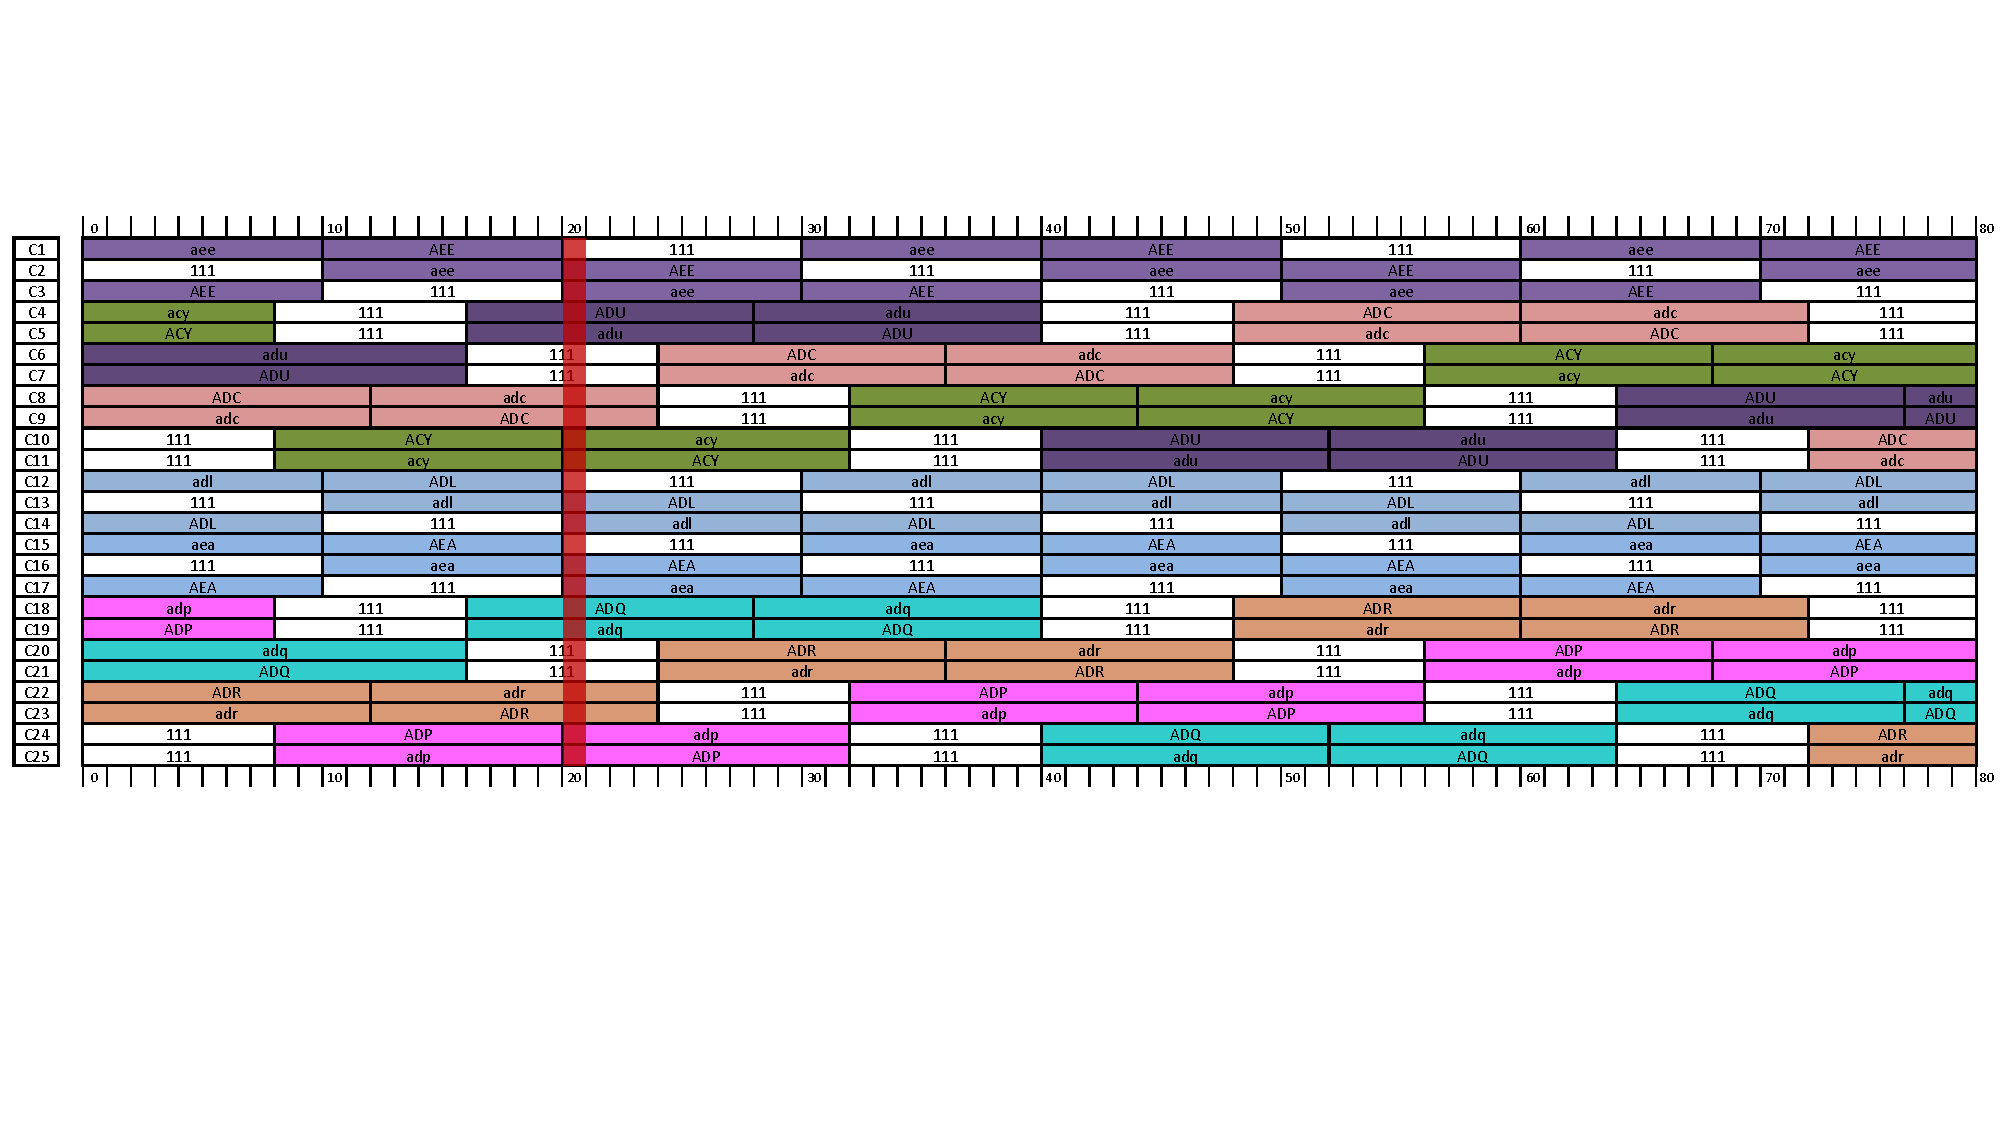
\includegraphics[width=\linewidth]{caso7/caso7-fase0}
	\caption{Planificación inicial del Caso 7}
	\label{fig:caso7-fase0}
\end{figure}

\begin{figure}[!h]
	\centering
	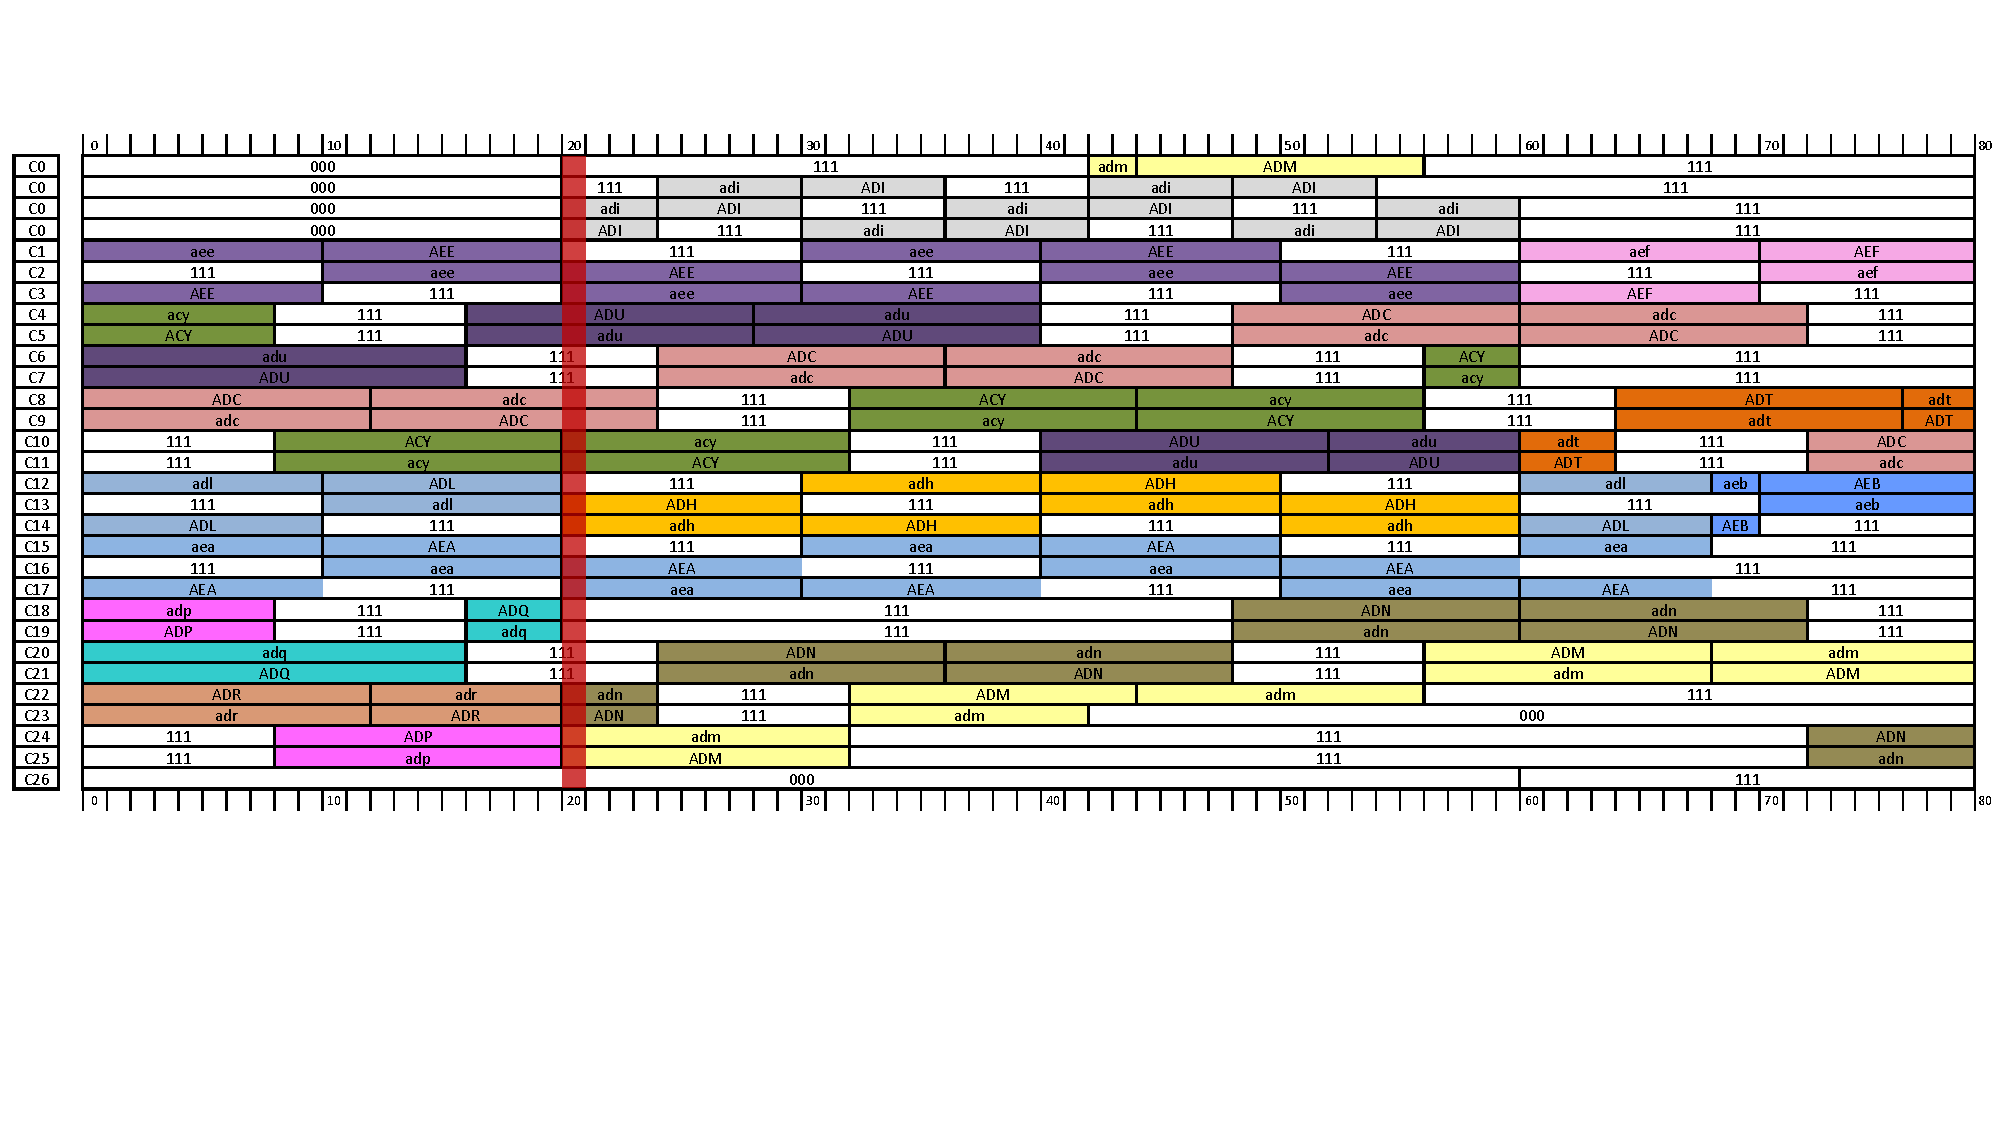
\includegraphics[width=\linewidth]{caso7/caso7-fase1}
	\caption{Solución inicial (\faseuno{}) para el Caso 7}
	\label{fig:caso7-fase1}
\end{figure}

\begin{figure}[!h]
	\centering
	\includegraphics[width=\linewidth]{caso7/caso7-fase2-vns}
	\caption{Solución final (\fasedos{}) para el Caso 7}
	\label{fig:caso7-fase2}
\end{figure}

\FloatBarrier
\newpage
\subsection{Caso 8}

\begin{figure}[!h]
	\centering
	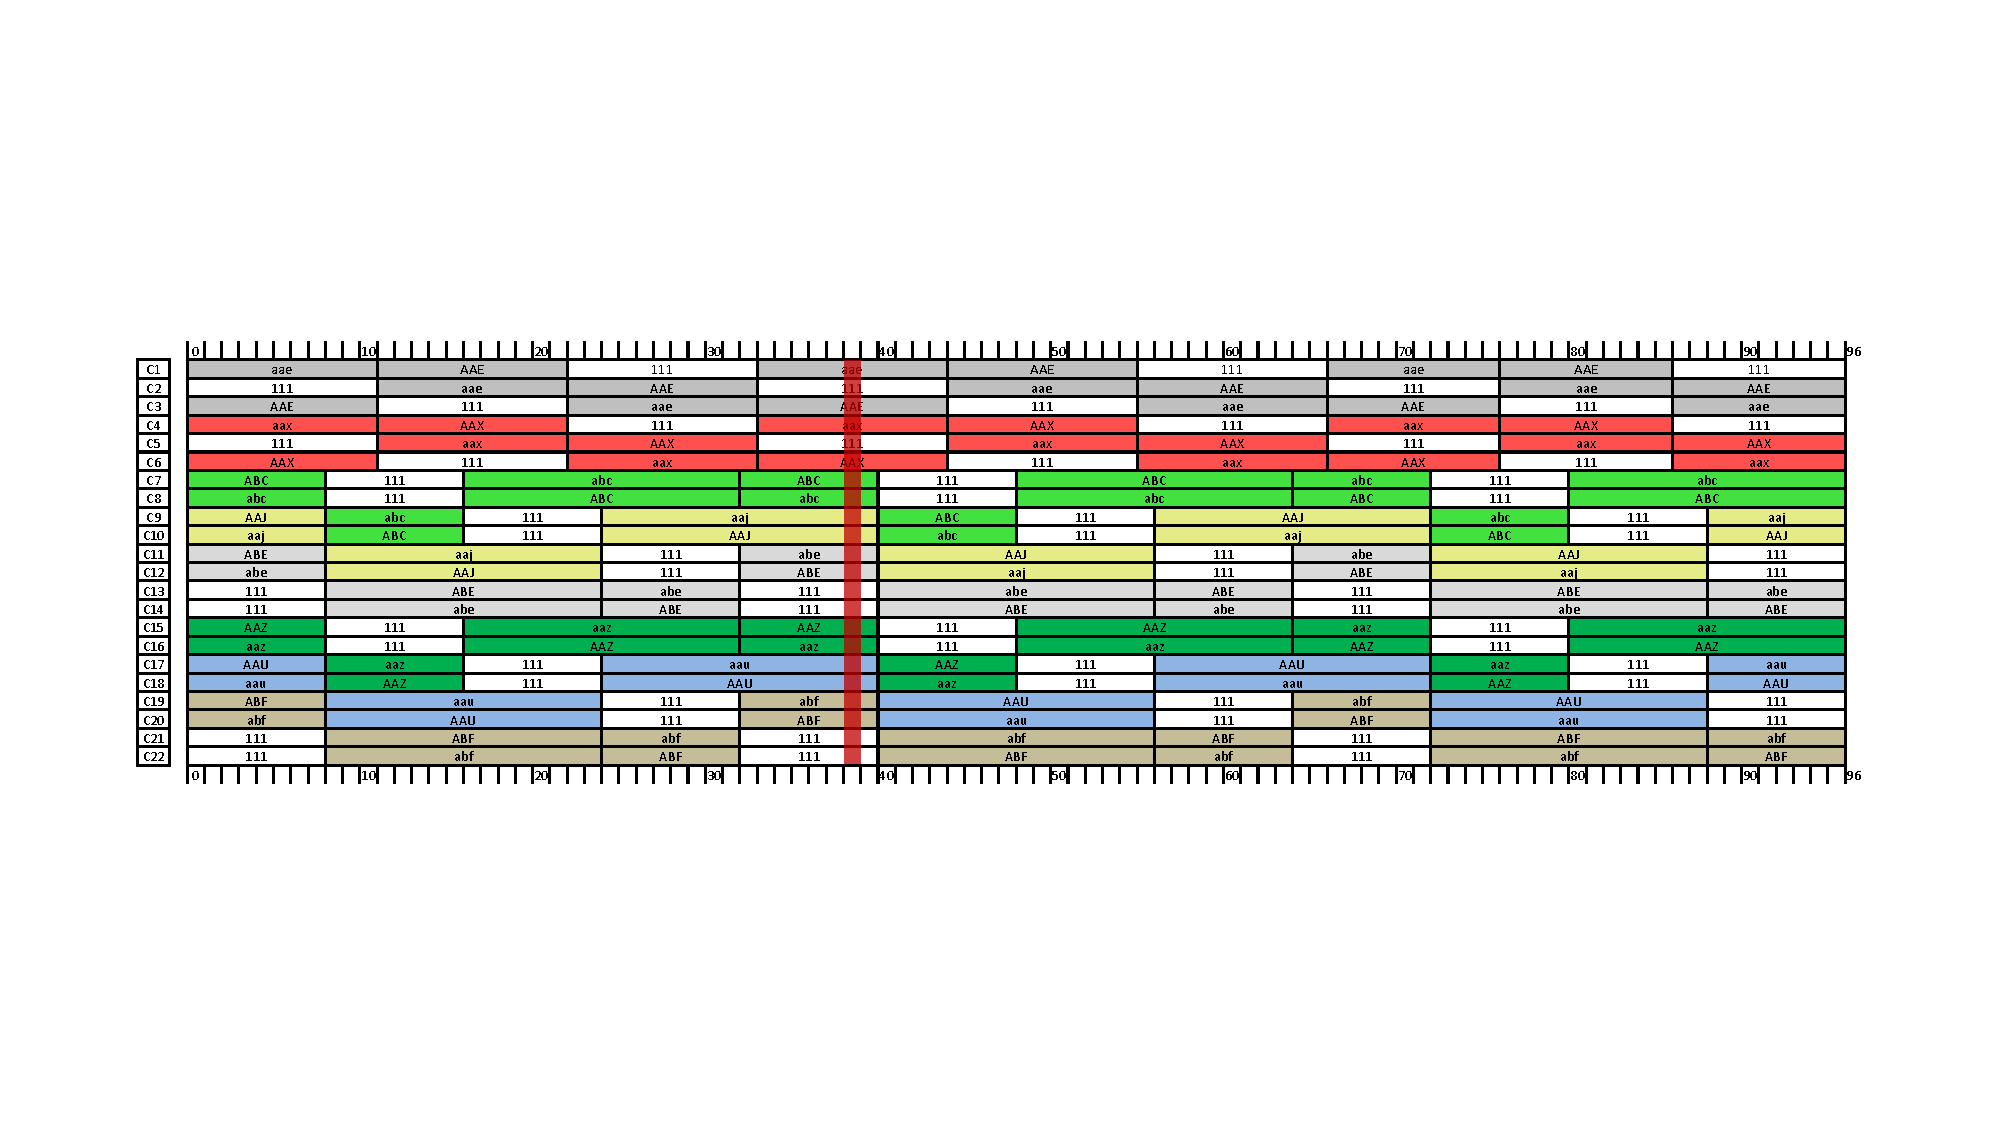
\includegraphics[width=\linewidth]{caso8/caso8-fase0}
	\caption{Planificación inicial del Caso 8}
	\label{fig:caso8-fase0}
\end{figure}

\begin{figure}[!h]
	\centering
	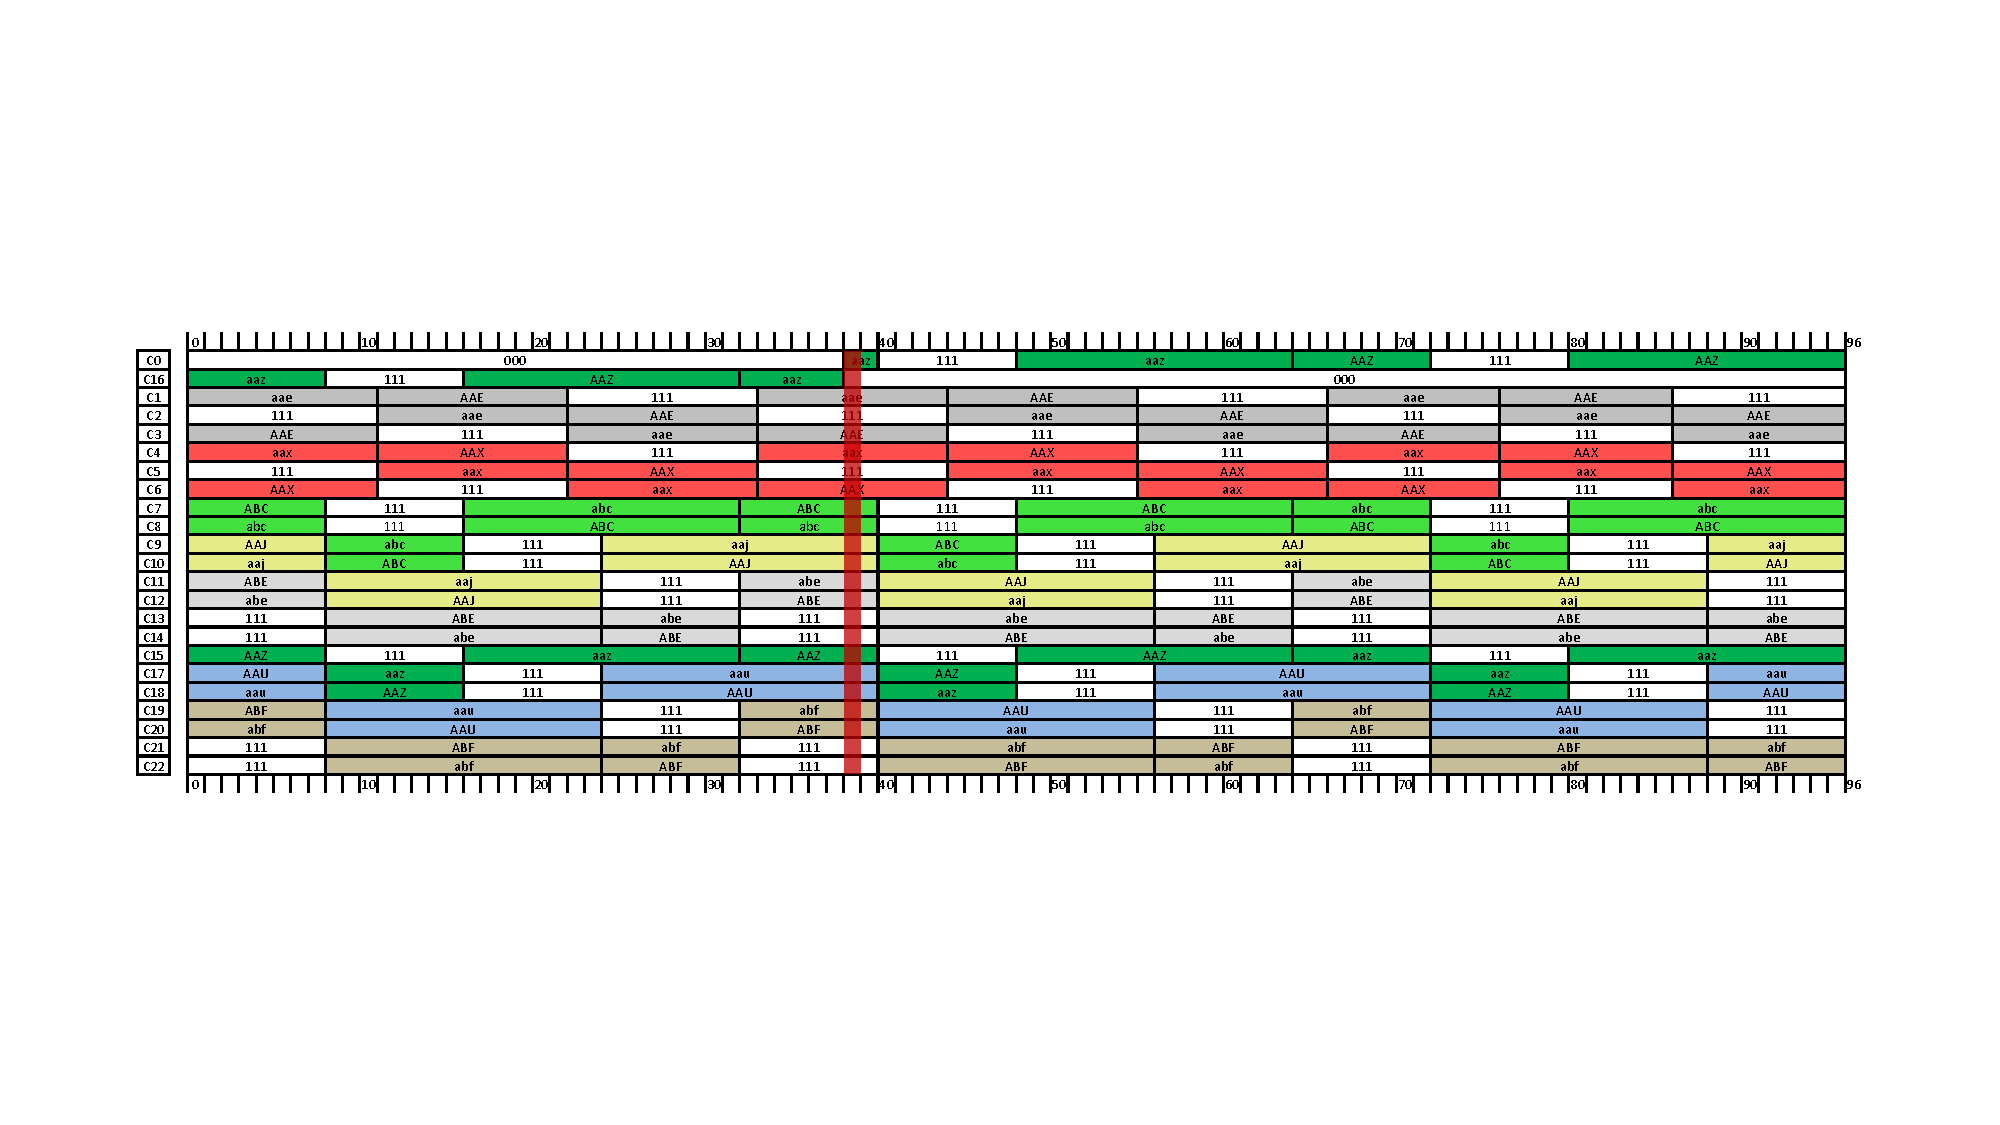
\includegraphics[width=\linewidth]{caso8/caso8-fase1}
	\caption{Solución inicial (\faseuno{}) para el Caso 8}
	\label{fig:caso8-fase1}
\end{figure}

\begin{figure}[!h]
	\centering
	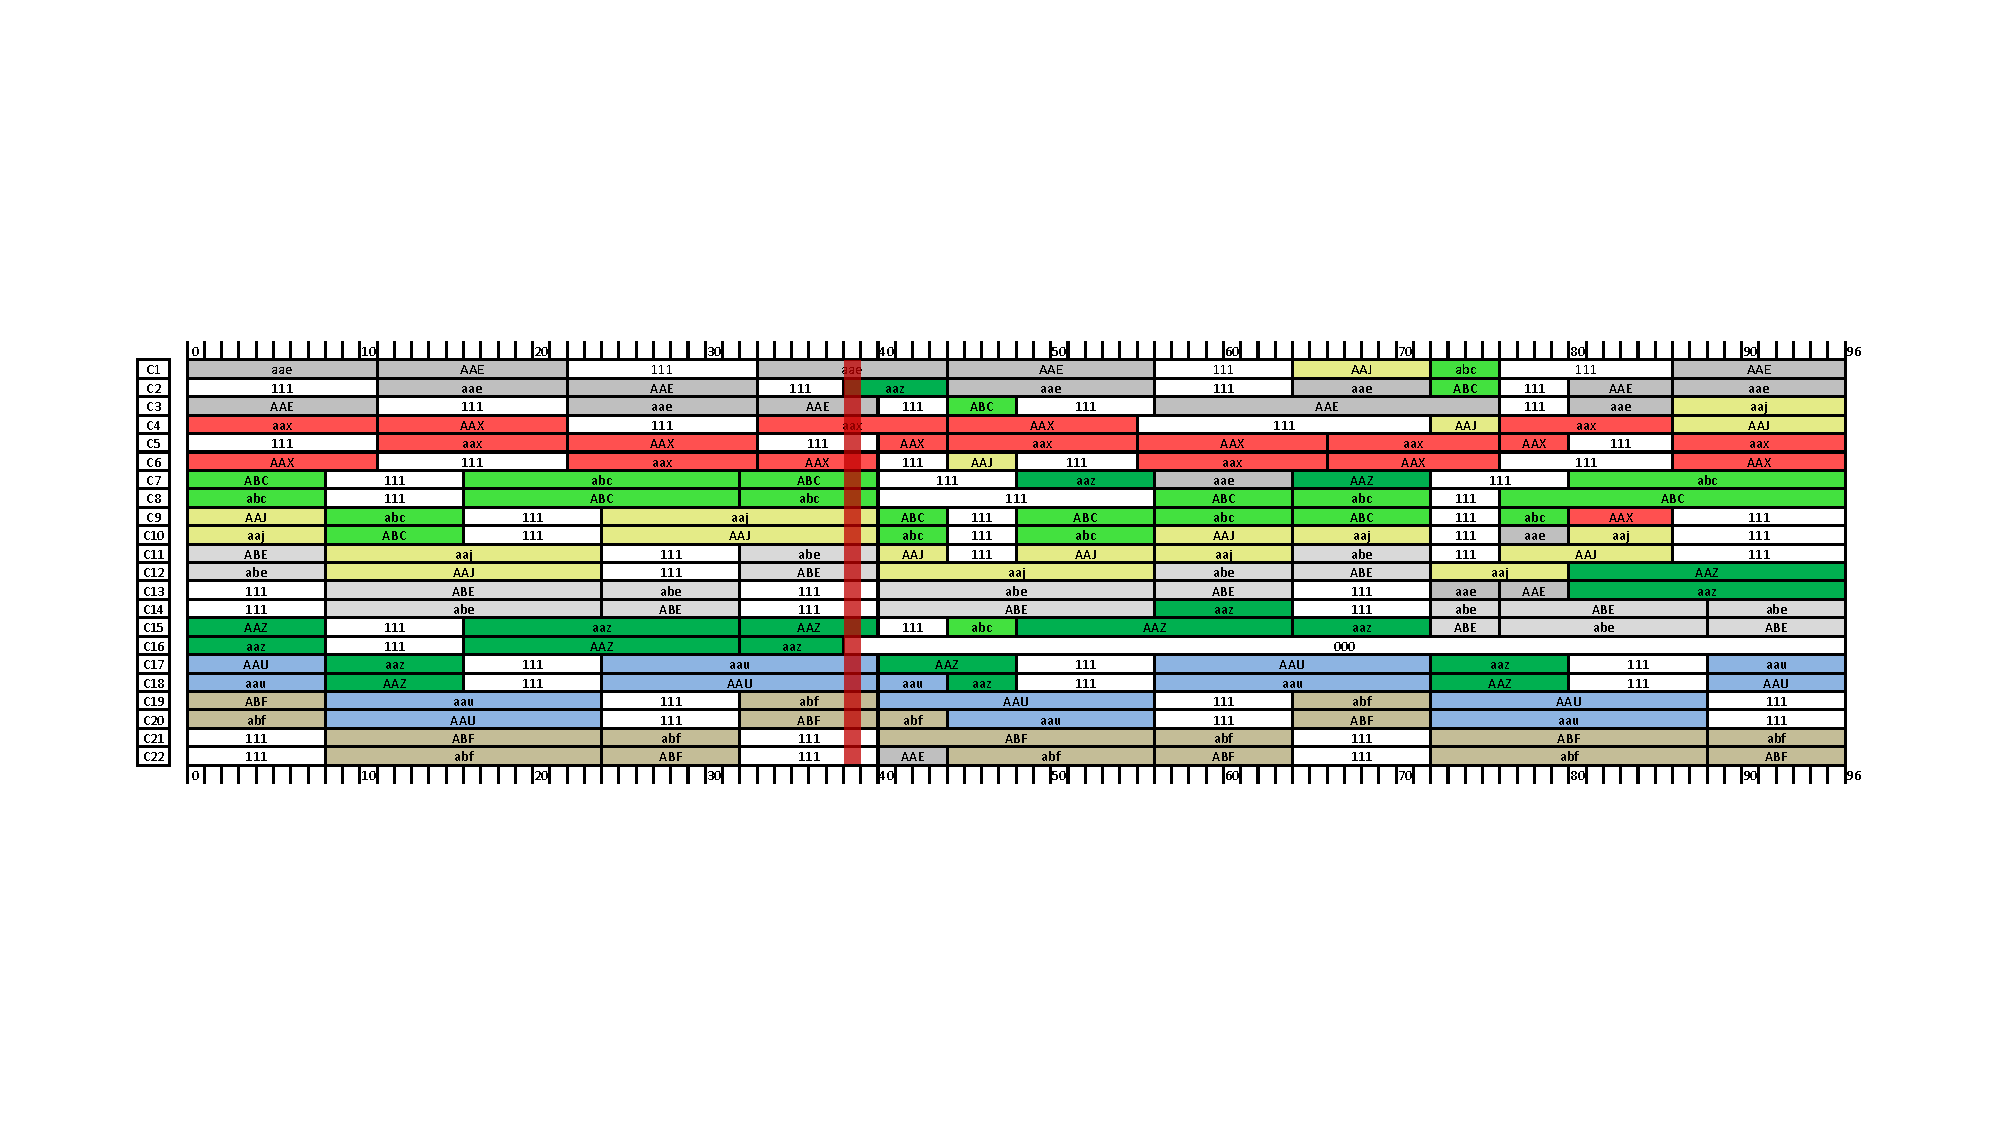
\includegraphics[width=\linewidth]{caso8/caso8-fase2}
	\caption{Solución final (\fasedos{}) para el Caso 8}
	\label{fig:caso8-fase2}
\end{figure}

\FloatBarrier
\newpage
\subsection{Caso 9}

La planificación inicial es la misma que la del Caso 8, cambiando el slot del momento del cambio.

\begin{figure}[!h]
	\centering
	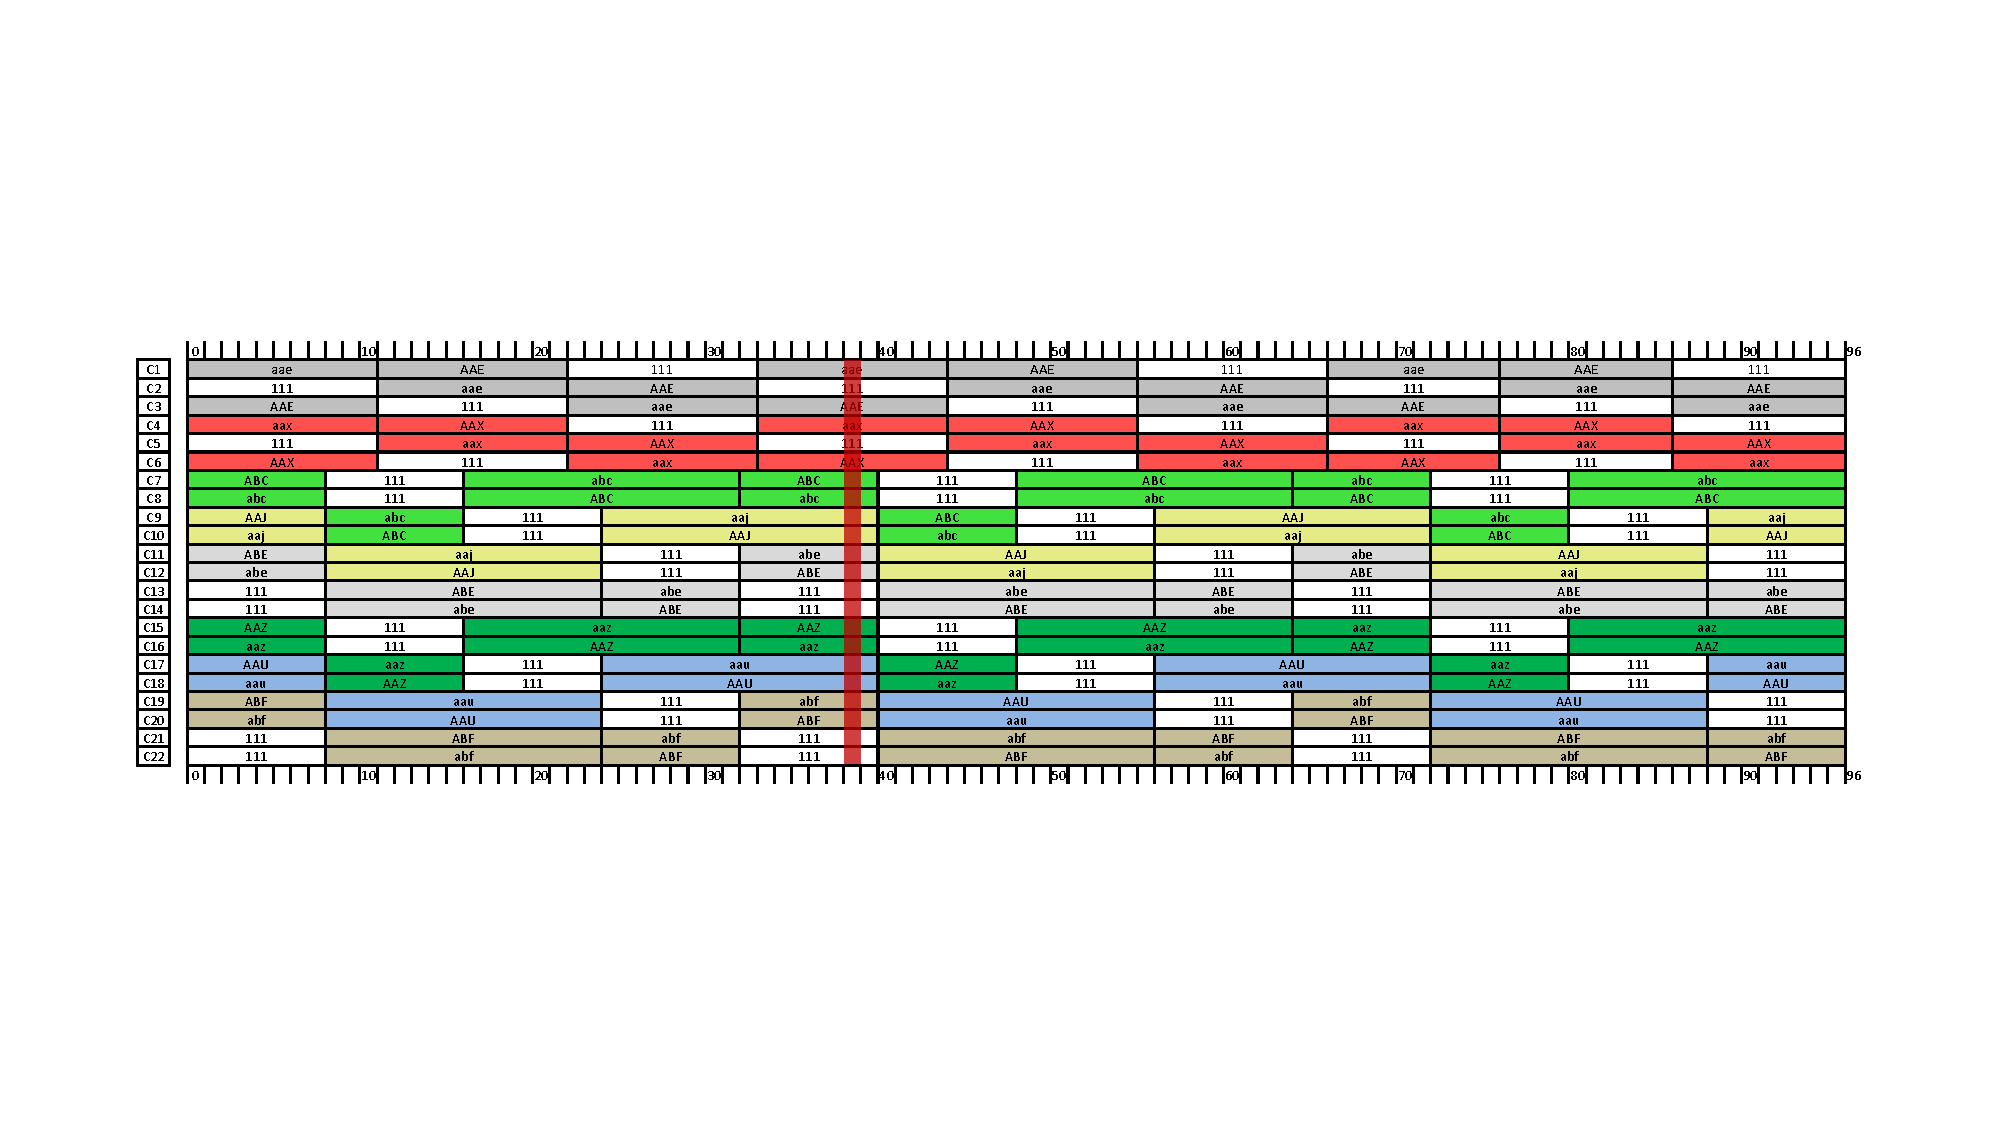
\includegraphics[width=\linewidth]{caso9/caso9-fase0}
	\caption{Planificación inicial del Caso 9}
	\label{fig:caso9-fase0}
\end{figure}

\begin{figure}[!h]
	\centering
	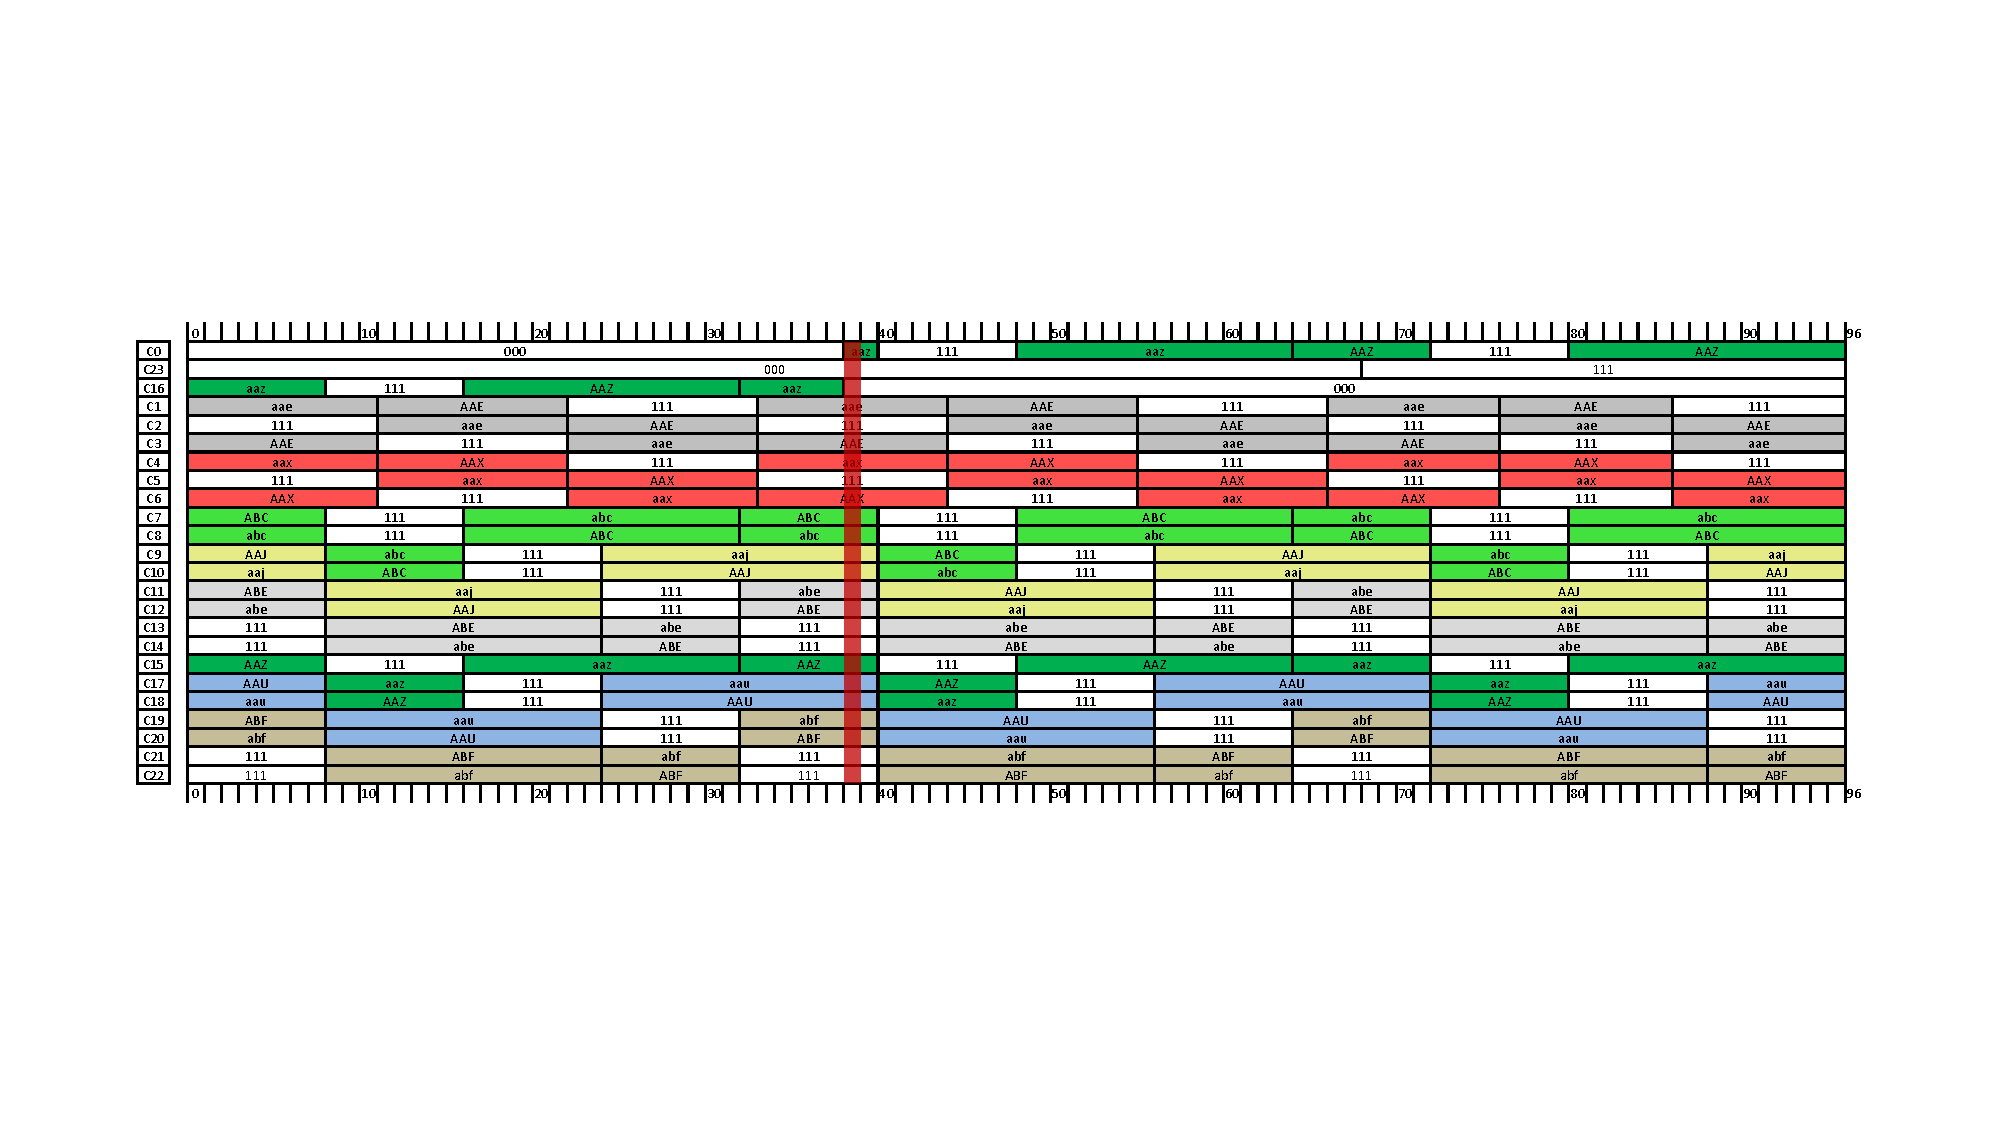
\includegraphics[width=\linewidth]{caso9/caso9-fase1}
	\caption{Solución inicial (\faseuno{}) para el Caso 9}
	\label{fig:caso9-fase1}
\end{figure}

\begin{figure}[!h]
	\centering
	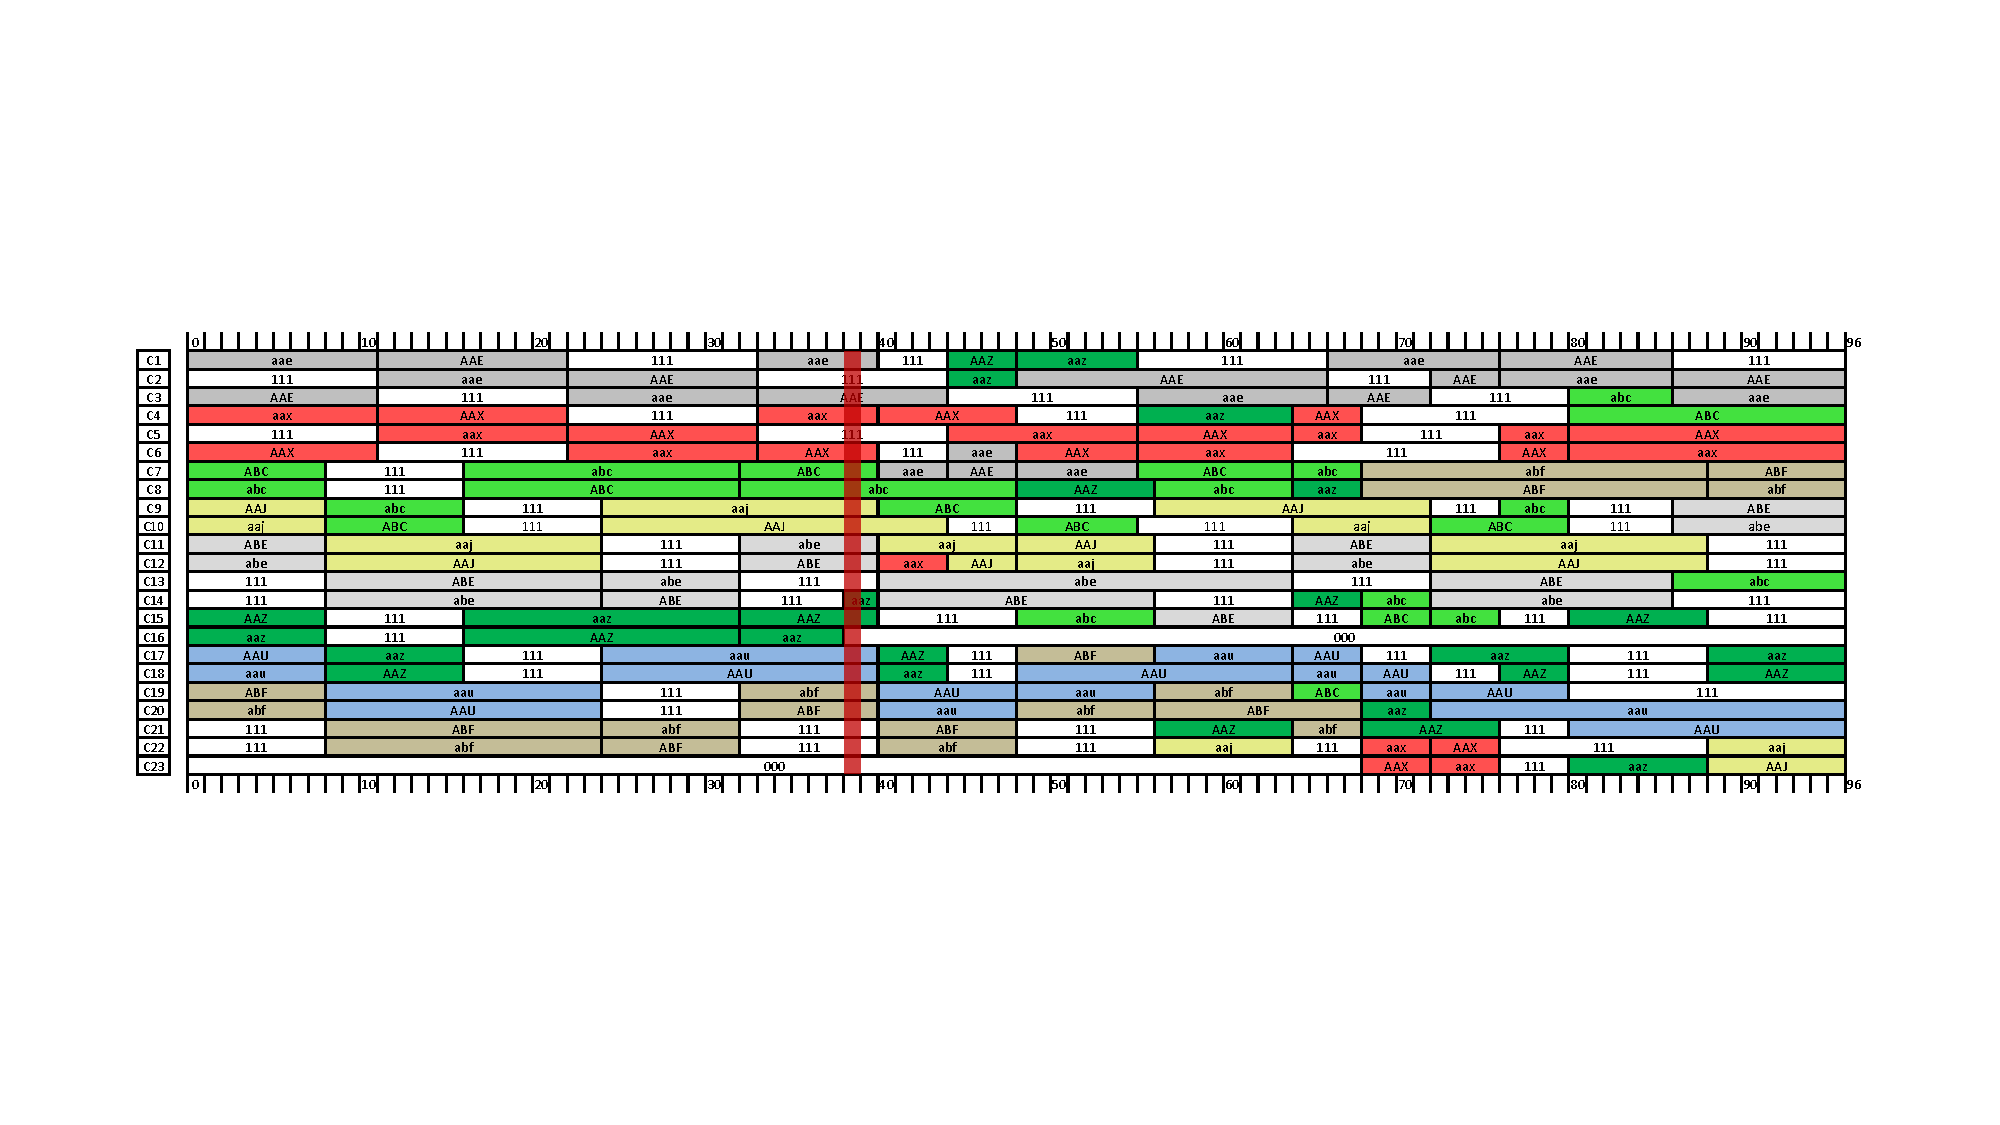
\includegraphics[width=\linewidth]{caso9/caso9-fase2}
	\caption{Solución final (\fasedos{}) para el Caso 9}
	\label{fig:caso9-fase2}
\end{figure}
